% 
% exemplo genérico de uso da classe iiufrgs.cls
% $Id: iiufrgs.tex,v 1.1.1.1 2005/01/18 23:54:42 avila Exp $
% 
% This is an example file and is hereby explicitly put in the
% public domain.
% 
\documentclass[cic,tc]{iiufrgs}
% Para usar o modelo, deve-se informar o programa e o tipo de documento.
% Programas :
% * cic       -- Graduação em Ciência da Computação
% * ecp       -- Graduação em Ciência da Computação
% * ppgc      -- Programa de Pós Graduação em Computação
% * pgmigro   -- Programa de Pós Graduação em Microeletrônica
% 
% Tipos de Documento:
% * tc                -- Trabalhos de Conclusão (apenas cic e ecp)
% * diss ou mestrado  -- Dissertações de Mestrado (ppgc e pgmicro)
% * tese ou doutorado -- Teses de Doutorado (ppgc e pgmicro)
% * ti                -- Trabalho Individual (ppgc e pgmicro)
% 
% Outras Opções:
% * english    -- para textos em inglês
% * openright  -- Força início de capítulos em páginas ímpares (padrão da
% biblioteca)
% * oneside    -- Desliga frente-e-verso
% * nominatalocal -- Lê os dados da nominata do arquivo nominatalocal.def


% Use unicode
\usepackage[utf8]{inputenc}   % pacote para acentuação

% Necessário para incluir figuras
\usepackage{graphicx}         % pacote para importar figuras

\usepackage{times}            % pacote para usar fonte Adobe Times
% \usepackage{palatino}
% \usepackage{mathptmx}       % p/ usar fonte Adobe Times nas fórmulas
\usepackage{amsfonts}
\usepackage{amsmath}
\usepackage{bm}
\usepackage{amsthm}      % Teoremas
\usepackage{thmtools}    % Front end para amsthm (\declaretheorem)
\usepackage{icomma}
\usepackage{listings}
\usepackage{tcolorbox}

\newcommand{\lstfont}[1]{\color{#1}\scriptsize\ttfamily}

\declaretheorem[style=definition,name=Definição,parent=chapter,qed=\textemdash]{definicao}
\declaretheorem[style=plain,name=Teorema,qed=\textnormal{\textemdash}]{teorema}
\declaretheorem[style=plain,name=Axioma,qed=\textnormal{\textemdash}]{axioma}

\usepackage[alf,abnt-emphasize=bf]{abntex2cite}	% pacote para usar citações abnt

\usepackage[portuguese,ruled,vlined,boxed]{algorithm2e}
\renewcommand{\algorithmautorefname}{Algoritmo}% para utilizar \autoref

\def\SPSB#1#2{\rlap{\textsuperscript{#1}}\SB{#2}}
\def\SP#1{\textsuperscript{#1}}
\def\SB#1{\textsubscript{#1}}

\renewcommand{\vec}[1]{\bm{#1}}
\newcommand{\mat}[1]{\bm{#1}}
\newcommand{\reg}{\textsuperscript{\textregistered}}

\usepackage{mathtools}
\DeclarePairedDelimiter{\ceil}{\lceil}{\rceil}
\DeclarePairedDelimiter{\floor}{\lfloor}{\rfloor}


\lstset{
    language=[ANSI]C++,
    showstringspaces=false,
    backgroundcolor=\color{white},
    basicstyle=\lstfont{black},
    identifierstyle=\lstfont{black},
    keywordstyle=\lstfont{blue!95},
    numberstyle=\lstfont{black},
    stringstyle=\lstfont{cyan},
    commentstyle=\lstfont{green!90},
    emph={
        cudaMalloc, cudaFree,
        __global__, __shared__, __device__, __host__,
        __syncthreads,
    },
    emphstyle={\lstfont{green!60!black}}
}


% 
% Informações gerais
% 
\title{Utilização de compressed sensing para compressão de frames e transmissão de vídeos em tempo real.}

\author{Sachser}{Eduardo}
% alguns documentos podem ter varios autores:
% \author{Flaumann}{Frida Gutenberg}
% \author{Flaumann}{Klaus Gutenberg}

% orientador e co-orientador são opcionais (não diga isso pra eles :))
\advisor[Prof.~Dr.]{Oliveira Neto}{Manuel Menezes de }
% \coadvisor[Prof.~Dr.]{Knuth}{Donald Ervin}

% a data deve ser a da defesa; se nao especificada, são gerados
% mes e ano correntes
% \date{maio}{2001}

% o local de realização do trabalho pode ser especificado (ex. para TCs)
% com o comando \location:
% \location{Itaquaquecetuba}{SP}

% itens individuais da nominata podem ser redefinidos com os comandos
% abaixo:
% \renewcommand{\nominataReit}{Prof\textsuperscript{a}.~Wrana Maria Panizzi}
% \renewcommand{\nominataReitname}{Reitora}
% \renewcommand{\nominataPRE}{Prof.~Jos{\'e} Carlos Ferraz Hennemann}
% \renewcommand{\nominataPREname}{Pr{\'o}-Reitor de Ensino}
\renewcommand{\nominataPRAPG}{Prof.~Vladimir Pinheiro do Nascimento}
% \renewcommand{\nominataPRAPGname}{Pr{\'o}-Reitora Adjunta de P{\'o}s-Gradua{\c{c}}{\~a}o}
% \renewcommand{\nominataDir}{Prof.~Philippe Olivier Alexandre Navaux}
% \renewcommand{\nominataDirname}{Diretor do Instituto de Inform{\'a}tica}
\renewcommand{\nominataCoord}{Prof.~Sérgio Luis Cechin}
% \renewcommand{\nominataCoordname}{Coordenador do PPGC}
% \renewcommand{\nominataBibchefe}{Beatriz Regina Bastos Haro}
% \renewcommand{\nominataBibchefename}{Bibliotec{\'a}ria-chefe do Instituto de Inform{\'a}tica}
% \renewcommand{\nominataChefeINA}{Prof.~Jos{\'e} Valdeni de Lima}
% \renewcommand{\nominataChefeINAname}{Chefe do \deptINA}
% \renewcommand{\nominataChefeINT}{Prof.~Leila Ribeiro}
% \renewcommand{\nominataChefeINTname}{Chefe do \deptINT}

% A seguir são apresentados comandos específicos para alguns
% tipos de documentos.

% Relatório de Pesquisa [rp]:
% \rp{123}             % numero do rp
% \financ{CNPq, CAPES} % orgaos financiadores

% Trabalho Individual [ti]:
% \ti{123}     % numero do TI
% \ti[II]{456} % no caso de ser o segundo TI

% Monografias de Especialização [espec]:
% \espec{Redes e Sistemas Distribuídos}      % nome do curso
% \coord[Profa.~Dra.]{Weber}{Taisy da Silva} % coordenador do curso
% \dept{INA}                                 % departamento relacionado

% 
% palavras-chave
% iniciar todas com letras minúsculas, exceto no caso de abreviaturas
% 
\keyword{Compressed Sensing}
\keyword{Compressed Sensing}
\keyword{Compressive Sampling}
\keyword{Real Time}
\keyword{Video}
\keyword{UFRGS}

%\settowidth{\seclen}{1.10~}

% 
% inicio do documento
% 
\begin{document}

% folha de rosto
% às vezes é necessário redefinir algum comando logo antes de produzir
% a folha de rosto:
% \renewcommand{\coordname}{Coordenadora do Curso}
\maketitle

% dedicatoria
% \clearpage
% \begin{flushright}
%     \mbox{}\vfill
%     {\sffamily\itshape
%       ``If I have seen farther than others,\\
%       it is because I stood on the shoulders of giants.''\\}
%     --- \textsc{Sir~Isaac Newton}
% \end{flushright}

% agradecimentos
%\chapter*{Agradecimentos}
%Agradeço ao \LaTeX\ por não ter vírus de macro\ldots



% resumo na língua do documento
\begin{abstract}
    Deve ser feito ainda.
\end{abstract}

% resumo na outra língua
% como parametros devem ser passados o titulo e as palavras-chave
% na outra língua, separadas por vírgulas
\begin{englishabstract}{Translate title to english.}{Compressed Sensing. Compressive Sensing. UFRGS}
    Must be done yet.
\end{englishabstract}

% lista de figuras
\listoffigures

% lista de tabelas
\listoftables

% lista de abreviaturas e siglas
% o parametro deve ser a abreviatura mais longa
\begin{listofabbrv}{CoSaMP}
    \item[RIP] Restricted Isometric Property
    \item[OMP] Orthogonal Matching Pursuit
    \item[CoSaMP] Compressive Sampling Matching Pursuit 
    \item[ODL] Online Dictionary Learning 
    \item[DCT] Discrete Cosine Transform 
    \item[GPU] Graphical Processing Unit
\end{listofabbrv}

% idem para a lista de símbolos
% \begin{listofsymbols}{$\alpha\beta\pi\omega$}
%     \item[$\sum{\frac{a}{b}}$] Somatório do produtório
%     \item[$\alpha\beta\pi\omega$] Fator de inconstância do resultado
% \end{listofsymbols}

% sumario
\tableofcontents

% aqui comeca o texto propriamente dito

% introducao
\chapter{Introdução}

\chapter{Referencial Teórico}

\section{Introdução a Sinais e Sistemas}
O trabalho apresentará uma metodologia para compressão de vídeos.
Porém, vídeos são, particularmente, uma sequência de imagens.
Já imagens, por sua vez, são um exemplo de sinais bidimensionais.
Vídeos, portanto, sinais tridimensionais.
Fica claro, a partir do posto acima, que há a necessidade de observar-se 
o que é um sinal e alguns resultados importantes, primeiramente, para 
em seguida aprimorarem-se os estudos acerca de outros conceitos.

"Um sinal é formalmente definido como uma função de uma ou mais variáveis, 
a qual veicula informações sobre a natureza de um fenômeno físico" \cite{haykin2001sinais}.
Também segundo \citet{haykin2001sinais}, os sinais são chamados unidimensionais quando
dependem de apenas uma variável, e multidimensionais quando dependem de mais que uma.
Exemplo de multidimensionais foram citadas anteriormente, imagens e vídeos. 
Já unidimensionais, podemos tomar como exemplo os sinais de som, dependentes apenas da variável tempo.

Além disso, temos de definir o que é um sistema. 
Segundo \citet{haykin2001sinais}, "Um sistema é definido como uma entidade que manipula
um ou mais sinais para realizar uma função, produzindo novos sinais".
Um exemplo simples poderia ser o controle de volume de um aparelho de som,
que gera um novo sinal proporcional ao sinal de entrada.
Podemos considerar sistemas bem mais complexos também, como um reconhecedor 
de faces, que precisa tomar como sinais as faces já conhecidas e a que se 
deseja reconhecer, e fornece como saída o nome ou as informações da face reconhecida.

Sinais podem ser contínuos, ou analógicos, ou digitais.
Na verdade, em geral, sinais da natureza são contínuos, mas são digitalizados 
para que seja possível armazenamento, envio e processamento por meios digitais.
Dessa forma, \citet{haykin2001sinais} apresenta os passos geralmente executados 
para digitalizar sinais analógicos:
\begin{enumerate}
    \item \emph{Amostragem:} O sinal analógico é amostrado com determinada taxa de amostragem.
    \item \emph{Quantização:} Cada uma das amostras é transformada para um valor digital em um intervalo definido.
    \item \emph{Codificação:} Os valores quantizados são salvos de alguma forma.
    \item \emph{Redundância:} Podem ser geradas informações de redundância para armazenamento do sinal.
\end{enumerate} 

De uma forma geral, a aquisição ou até mesmo a transmissão de um sinal podem conter ruído.
Dessa forma, pode se imaginar que um sinal amostrado é composto pelo próprio sinal somado ao ruído,
$\vec{f} = \vec{y} + \vec{e}$, no qual $\vec{f}$ é a amostragem, $\vec{y}$ é o sinal real, 
e $\vec{e}$ é o erro.


Uma definição importante para o prosseguimento do trabalho é a de energia de um sinal $\vec{f} \in \mathbb{R}^m$,
$E$, como segue:
\begin{equation}
    E = \sum_{i=1}^m \vec{f_i}^2
\end{equation}

Por fim, um resultado clássico sobre amostragem de sinais no domínio tempo, o teorema Shannon-Nyquist.
\begin{teorema}
    \cite{NyquistSampling}.
    Um sinal contínuo pode ser apropriadamente amostrado somente se ele não contiver 
    componentes em frequência $f_{max}$ acima de metade da frequência de amostragem $f_s$.
    \begin{equation*}
        f_{max} \le \frac{f_s}{2}.
    \end{equation*}
\end{teorema}

A partir desse pequeno resumo focado em amostragem de sinais digitais,
as próximas seções utilizarão os conceitos apresentados para formularem outros novos.

\section{Compressed Sensing}
\subsection{O modelo de Compressed Sensing}
\textit{Compressed Sensing (CS)} ou \textit{Compressive Sampling} é um campo de estudo de sinais cujos
primeiros trabalhos surgiram a partir de 2006, a partir da análise de amostragens executadas em imagens de 
ressonância magnética. Essas amostragens eram de muito menor dimensionalidade do que a da imagem, o que 
fez com que os métodos conhecidos de processamento de sinais não tivessem boa acurácia.

"Muitos sinais de interesse possuem menos informação do que a dimensão do ambiente sugere"
\footnote{"Many signals of interest contain far less information than their ambient dimension suggests"}
(\citeauthor{chen2015compressed}, \citeyear{chen2015compressed}, p. 2, tradução própria).
As formas tradicionais de aquisição de sinais baseadas nos teoremas de Shannon e Nyquist acabam por causar o descarte
de boa parte da informação coletada durante a etapa de compressão. Tal fato traz a tona a pergunta: é possível haver 
uma forma de aquisição dos sinais na qual as amostras comprimidas são obtidas diretamente? 

O modelo de Compressed Sensing surgiu com esse intuito \cite{DonohoCS}. Trabalhos na área mostram que, para certas classes
de sinais, poucas amostras são necessárias para representar o sinal com acurácia \cite{chen2015compressed}.
Ou seja, Compressed Sensing busca encontrar quais tipos
de sinais podem ser amostrados de forma já comprimida e respostas de como fazê-lo.

De acordo com o modelo, um sinal $ \vec{f} $ em geral é um elemento de $ \mathbb{C}^d $. Amostragens são executadas na forma:
\begin{equation}
    y_i = \langle \vec{\phi_i}, \vec{f} \rangle \text{ para } i=1,2,...,m, 
\end{equation}
na qual $m \ll d$. Os vetores $\vec{\phi_i}$ são linhas de uma matriz $m \times d$ $\mathbf{\Phi}$, chamada matriz 
de amostragem. Assim, pode-se reescrever o vetor de amostragem como $\vec{y} = \mathbf{\Phi} \vec{f}$. Fica claro que, 
se $ m \ll d$, reconstruir $\vec{f}$ a partir de $\vec{y}$, sem assumir nada a mais, é um problema 
com infinitas soluções \cite{chen2015compressed}.

Uma importante consideração que CS faz é a de que os sinais de interesse possuem menos informação do que sugere a 
dimensão $d$. Uma forma de quantificar essa noção é a esparsidade, que pode ser definida como a quantidade de valores não
nulos $s$ de um sinal $\vec{f} \in \mathbb{C}^d$, também conhecida como norma $\ell_0$:
\begin{equation}
    \lVert \vec{f} \rVert_0 = s
\end{equation}

Considerando o mesmo sinal $\vec{f}$, diz-se que este é \textit{s-esparso}, quando, para dado um um valor $s$, $\vec{f}$
satisfaz a seguinte inequação:
\begin{equation}
    \label{eq:f0less}
    \lVert \vec{f} \rVert_0 \le s \ll d
\end{equation} 

Na prática, sinais não são usualmente encontrados esparsos, o que leva a definição de que \textit{sinais compressíveis}
são aqueles que obedecem a seguinte lei de decaimento exponencial:
\begin{equation}
    \label{eq:compressiblesignal}
    | f\SPSB{*}{k} | < R k^{-\frac{1}{q}},  
\end{equation}
tal que $\vec{f}^* $ é o rearranjo decrescente de $\vec{f}$, $R$ é uma constante positiva e $0< q < 1$. Percebe-se
que para valores bem pequenos de $q$ a compressibilidade se torna praticamente o mesmo que esparsidade. Se considerarmos
$\vec{f_s}$ o vetor com os $s$ maiores valores de $\vec{f}$ em magnitude, temos que, para sinais compressíveis $\vec{f}$ e 
$\vec{f_s}$:
\begin{equation}
    \lVert \vec{f} - \vec{f_s} \rVert_2 \le Rs^{\frac{1}{2} - \frac{1}{q}} \hspace{1em} \text{ e } \hspace{1em}
    \lVert \vec{f} - \vec{f_s} \rVert_1 \le Rs^{1 - \frac{1}{q}} 
\end{equation} 

Por fim, a definição \eqref{eq:f0less} exige que $\vec{f}$ seja esparso, ou seja, tenha $s$ coeficientes não nulos
no máximo. Por outro lado, $\vec{f}$ pode ser esparso em alguma outra base ortonormal $\mathbf{D}$, uma \textit{sparsifying basis} 
\cite{CandesDecoLinear}. Nesse caso, considera-se $\vec{f}$ s-esparso se:
\begin{equation}
    \vec{f} = \mathbf{D}\vec{x} \hspace{1em} \text{dado que} \hspace{1em} \lVert \vec{x} \rVert_0 \le s \ll d.
\end{equation}


\subsection{Mecanismos de Amostragem}
A partir das definições básicas do modelo, pode-se formular o problema básico de CS da seguinte forma:

Tomando um operador de amostragem $\mathbf{\Phi}$, mapeamento linear de $\mathbb{C}^d$ para algum espaço de dimensão 
$\mathbb{C}^m$, para recuperarmos um sinal $\vec{f}$ a partir de suas medidas $\vec{y} = \mathbf{\Phi} \vec{f}$, pode-se escrever
como um problema de minimização.
\begin{equation}
    \label{eq:problem}
    \vec{f}' = \underset{\vec{g} \in \mathbb{C}^d}{\text{argmin}} \lVert \vec{g} \rVert_0 \hspace{1em} \text{sujeito a} \hspace{1em}
    \mathbf{\Phi} \vec{g} = \vec{y} 
\end{equation}

A partir da formulação, se $\mathbf{\Phi}$ não mapeia 2 vetores esparsos quaisquer para a mesma imagem, ou seja,
se $\vec{f} \ne \vec{g} \rightarrow \mathbf{\Phi}\vec{f} \ne \mathbf{\Phi}\vec{g} $, então a solução $\vec{f}'$ recupera
$\vec{f}$, $\vec{f}' = \vec{f}$ \cite{chen2015compressed}. Esse problema, por outro lado, é intratável, e, em geral,
NP-difícil \cite{Mut05}.
Para que o operador de amostragem forneça o resultado anterior, ele deve ser \textit{incoerente}.
Dado um operador $\mathbf{\Phi}$ de colunas $\{ \vec{\phi_i} \}$  com norma unitária, define-se a sua coerência $\mu$
como a maior correlação entre suas colunas.
\begin{equation}
    \label{eq:coerence}
    \mu = \underset{i \ne j}{max}\langle \vec{\phi_i} , \vec{\phi_j} \rangle
\end{equation}

Fica definido, portanto, que um operador de amostragem é \textit{incoerente} quando a sua coerência $\mu$ é 
suficientemente pequena. Por exemplo, um operador de amostragem que seja uma base ortonormal é incoerente, bem como
operadores que sejam aproximadamente ortonormais para vetores esparsos.

Uma propriedade que captura a mesma ideia que o referido acima foi desenvolvida por \citet{CandesSignalRecovery}, chamada 
\textit{Restricted Isometry Property} (RIP). A constante de isometria restrita 
$\delta_s$ é a menor tal que:
\begin{equation}
    \label{eq:rip}
    (1 - \delta_s)\lVert \vec{f} \rVert\SPSB{2}{2} \le \lVert \mathbf{\Phi} \vec{f} \rVert \SPSB{2}{2} \le 
    (1 + \delta_s)\lVert \vec{f} \rVert\SPSB{2}{2} \hspace{1em} \text{para todo vetor s-esparso } \vec{f}.
\end{equation}

Diz-se que um operador de amostragem $\mathbf{\Phi}$ tem a RIP de ordem $s$ quando $\delta_s$ é suficientemente
pequeno, por exemplo, $\delta_s \le 0,1$.

A questão importante da RIP é descobrir qual o número de amostras $m$ é necessária e quais são as 
classes de matrizes que possuem a propriedade. Doi importantes exemplos de matrizes que satisfazem a RIP são
as seguintes \cite{chen2015compressed}: 
\begin{itemize}
    \item \textbf{Matrizes subgaussianas}: uma variável randômica $\mat{X}$ é subgaussiana se 
    $\mathbb{P}(|\mat{X}| > t) \le Ce^{-ct^2}$ para todo $t>0$ e constantes positivas $C$ e $c$. Ou seja,
    variáveis subgaussianas possuem distribuição de média aproximadamente $0$, e a maior parte dos valores
    próximos a média. Exemplos dessa distribuição são a própria distribuição Gaussiana e a matrizes de 
    Bernoulli, que possuem coeficientes $-1$ e $+1$ distribuídos com média $0$. \citet{Mendelson2008} provaram que
    se $\mat{\Phi} \in \mathbb{R}^{m\times d}$ é subgaussiana, então, com alta probabilidade, $\frac{1}{\sqrt{m}}\mat{\Phi}$
    satisfaz a RIP de ordem $s$ quando $m$ está na ordem de $s\log{d}$.
    \item \textbf{Matrizes parcialmente ortogonais limitadas}: dada uma matriz $d\times d$ ortogonal $\mat{\Psi}$
    cujos coeficientes são limitados por $\frac{C}{\sqrt{d}}$ para uma constante $C$. Uma matriz parcialmente
    ortogonal limitada $\mat{\Phi}$ é formada escolhendo $m$ colunas de $\mat{\Psi}$ randomicamente.
    Por exemplo, a matriz da transformada discreta de Fourier tem coeficientes limitados em $\frac{1}{\sqrt{d}}$,
    logo escolhendo $m$ linhas randomicamente tem-se uma matriz parcialmente ortogonal limitada.
    \citet{rudelson2008sparse} provaram que essas matrizes satisfazem RIP com alta probabilidade quando
    o número de medidas $m$ é na ordem de $s\log^4{d}$.
\end{itemize}


\subsection{Algoritmos aplicados ao modelo de Compressive Sensing}
\label{sec:csalgo}
Ao considerar-se a formulação do problema geral de CS apresentada na seção anterior, um dos resultados também apresentados
é de que o problema é NP-difícil. Sob essa ótica, diversas soluções alternativas foram desenvolvidas com 
o intuito de, através da solução de algum outro problema relacionado, ou do uso de alguma diferente estratégia, fosse possível 
chegar a uma solução ótima para a formulação de CS. 

Inicialmente, é necessário levar em consideração que nem sempre as amostras coletadas estão completamente corretas,
o que leva a um novo vetor de medidas, $\vec{y} = \mathbf{\Phi} \vec{f} + \vec{e}$, que considera o ruído de amostragem, 
ou vetor de erro, $\vec{e}$.

Além disso, é essencial definir as propriedades ideais de um método de recuperação
baseado em CS. Segundo \citet{chen2015compressed}, as propriedades são as seguintes:
\begin{itemize}
    \item \textbf{Amostragem não adaptativa:} Os operadoes de amostragem não devem ser dependentes do sinal. 
          Operadores que possuem RIP também possuem essa propriedade.
    \item \textbf{Número ótimo de amostras:} O número de amostras necessárias deve ser mínimo.
    \item \textbf{Garatia de Uniformidade:} Um único operador de amostragem deve ser suficiente para qualquer sinal.
    \item \textbf{Robustez:} O método deve ser estável e robusto em relação ao ruído, e possuir garantias 
          quanto ao erro.
    \item \textbf{Complexidade:} O algoritmo deve ser eficiente.
\end{itemize}

Buscando obedecer o maior número das propriedades citadas acima, alguns métodos e algoritmos surgiram. 
Nas subseções seguintes serão descritas duas metodologias que foram utilizadas para tal.

\subsubsection{Métodos baseados em otimização}
Essa metodologia, utilizada pelos primeiros trabalhos na área, utiliza uma relaxação convexa como forma
de chegar a solução do problema \eqref{eq:problem}. Ou seja, utiliza a norma $\ell_1$ ao invés da norma $\ell_0$,
de forma que o problema se torna convexo e solúvel através de métodos de programação linear.

Dessa forma, o problema relaxado para a norma $\ell_1$ fica como segue:
\begin{equation}
    \label{eq:probleml1}
    \vec{f'} = \underset{\vec{g} \in \mathbb{C}^d}{\text{argmin}} \lVert \vec{g} \rVert_1 \hspace{1em} \text{sujeito a} \hspace{1em}
    \lVert \mathbf{\Phi} \vec{g} - \vec{y} \rVert_2 \le \epsilon
\end{equation}
tal que $\lVert \vec{e} \rVert_2 \le \epsilon $.

A geometria da norma $\ell_1$ permite esparsidade, como pode-se ver no exemplo a seguir. Imaginando-se 
que a reta em verde retrata todas as possíveis soluções para um sinal $\vec{f} \in \mathbb{R}^2$, os pontos
mais esparsos da reta são $A=(0;1)$ e $B=(-1.\overline{6};0)$. A região em azul limita todos os pontos 
nos quais $\lVert\vec{p}\rVert_1 \le 1,0$, tal que $\vec{p} \in \mathbb{R}^2$. Nesse caso, o ponto $A$ é o 
de menor norma $\ell_1$ da reta, sendo essa a solução do problema \eqref{eq:probleml1} e, ao mesmo tempo, 
uma das possíveis soluções do problema \eqref{eq:problem}.
\begin{figure}[h]
    \caption{Minimização $\ell_1$ nos pontos da reta.}
    \begin{center}
        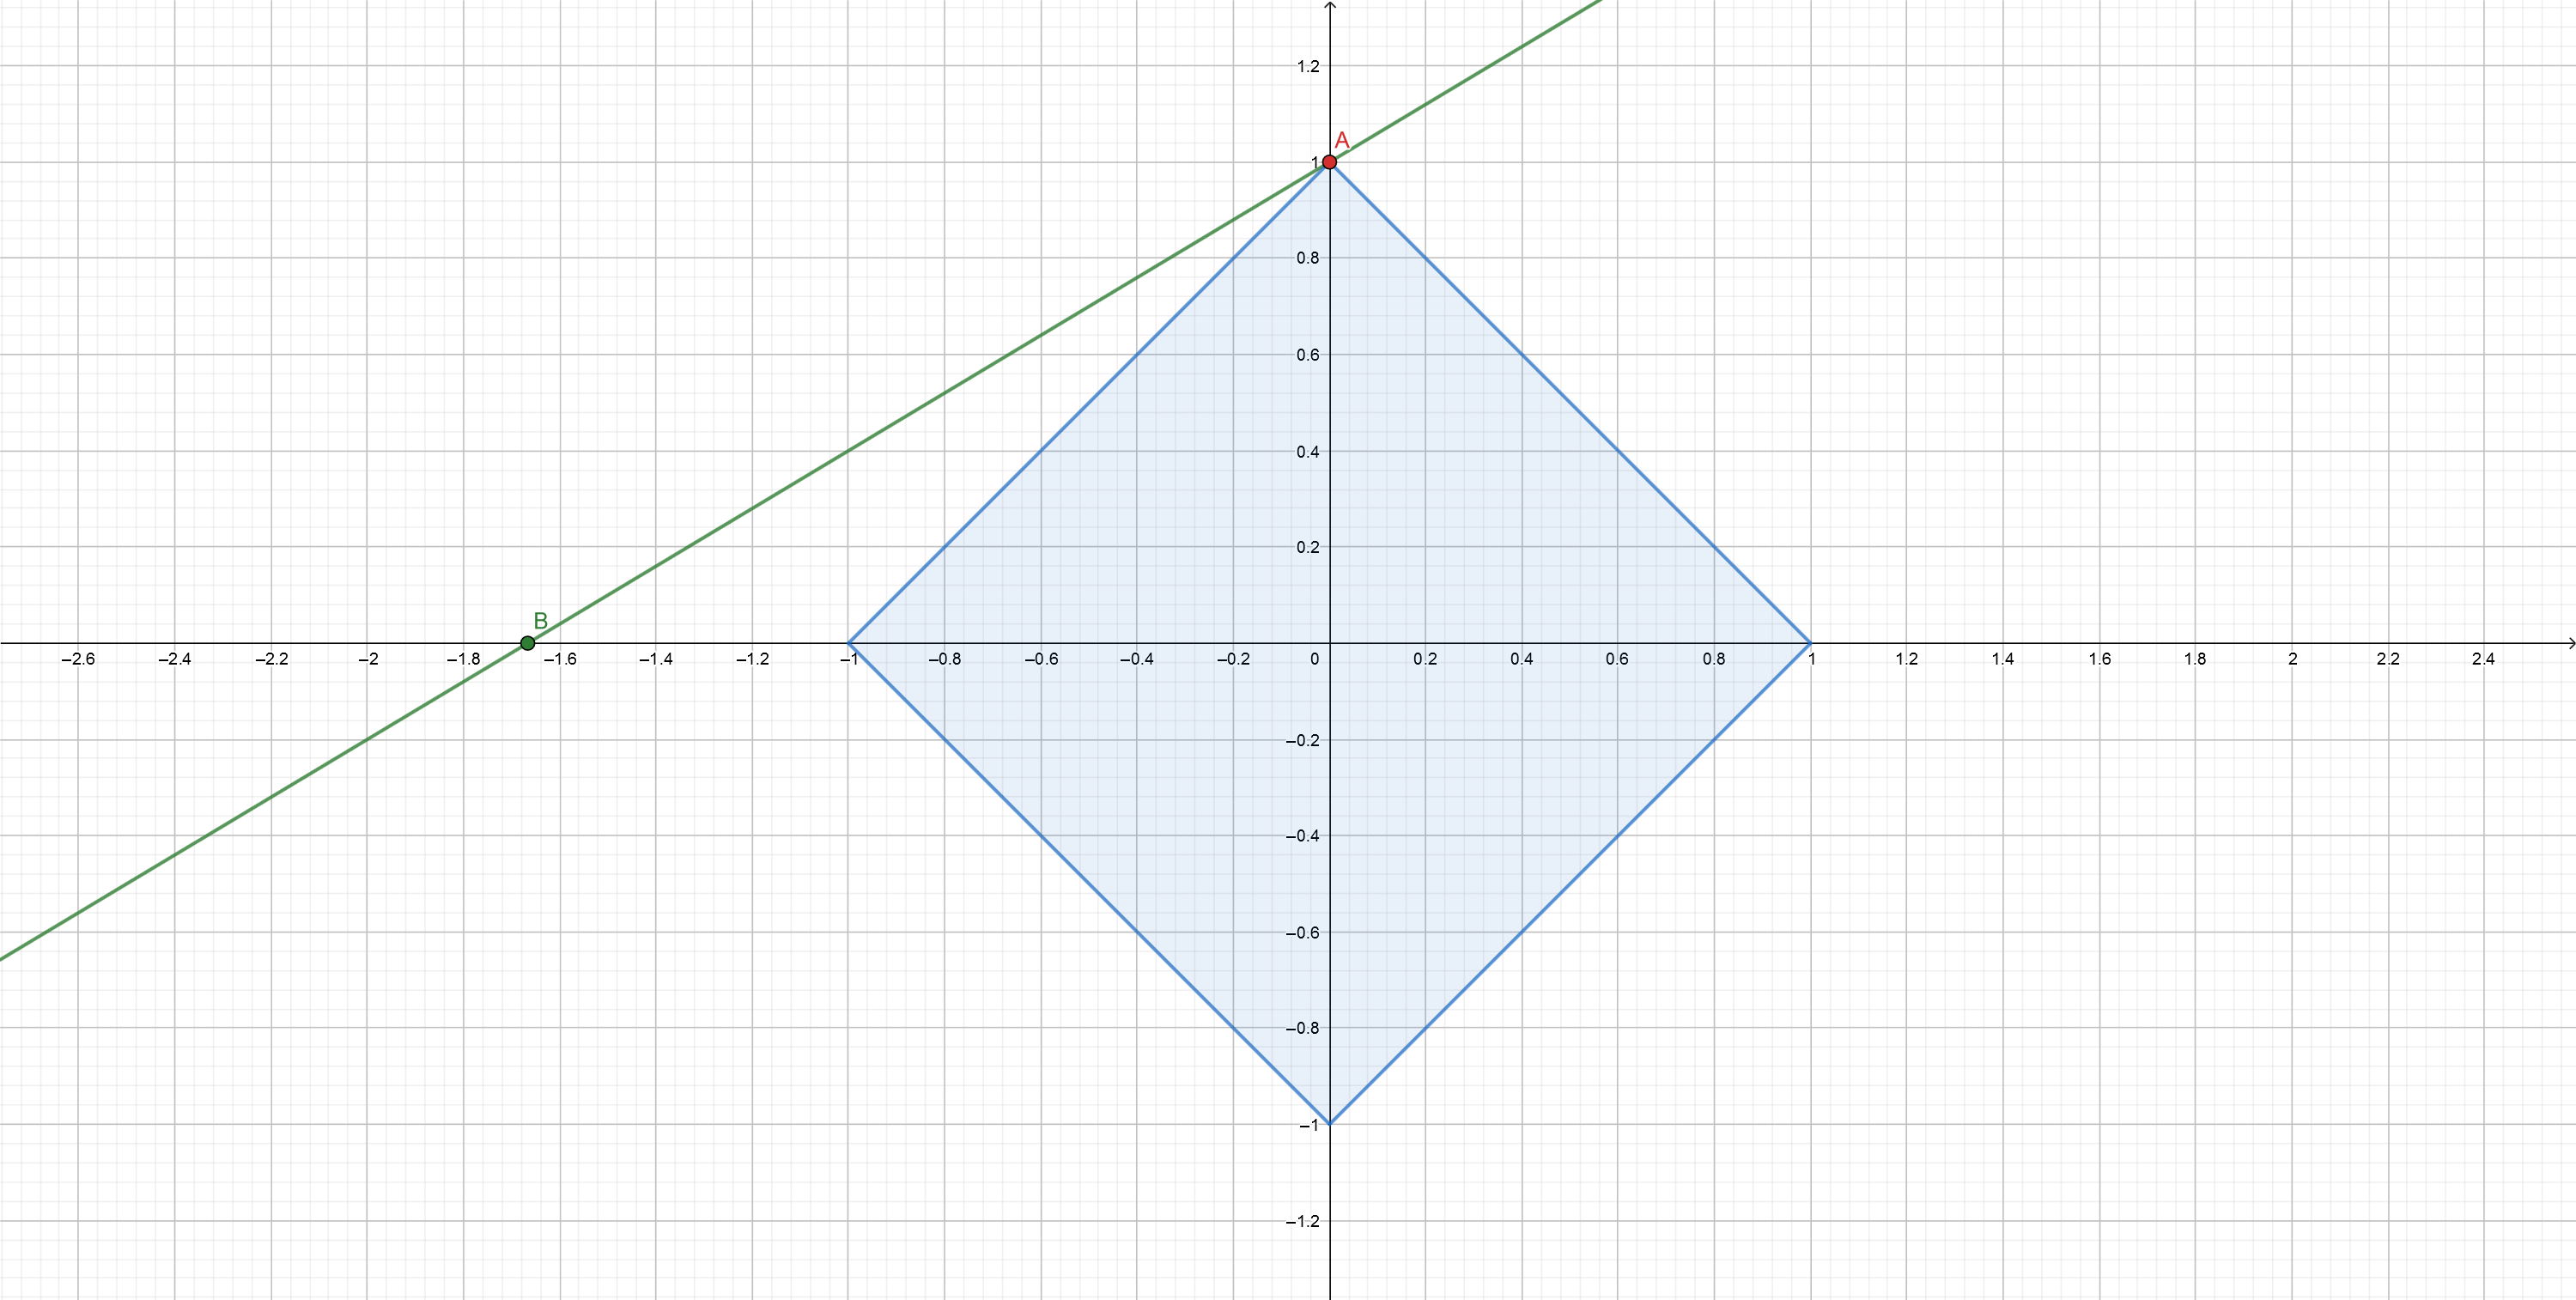
\includegraphics[width=0.9\textwidth]{img/l1ball}
    \end{center}
    \legend{Fonte: O Autor}
    \label{fig:l1ball}
\end{figure}

Candès, Romberg e Tao chegaram a resultados quanto a garantias para os limites de erro, baseado na 
intensidade do ruído, como segue.
\begin{teorema}
    \cite{candes2006stable}. 
    Dado um operador de amostragem $\mathbf{\Phi}$ que satisfaz a RIP.
    Então, para qualquer sinal $\vec{f}$ e sua amostragem ruidosa $\vec{y} = \mathbf{\Phi}\vec{f} + \vec{e}$, 
    tal que $\lVert \vec{e} \rVert_2 \le \epsilon$, a solução $\vec{f}'$ de \eqref{eq:probleml1} satisfaz:
    \begin{equation*}
        \lVert \vec{f}' - \vec{f} \rVert_2 \le C \left[ \epsilon + \frac{\lVert \vec{f} - \vec{f_s} \rVert_1}{\sqrt{s}} \right],
    \end{equation*}
    tal que $\vec{f_s}$ denota o vetor com os $s$ maiores coeficientes em magnitude de $\vec{f}$ e $C$ é uma
    constante tal que $C \ge 0$.
\end{teorema}

\subsubsection{Métodos utilizando algoritmos gulosos}
\label{sec:greedy}
Depois da formalização do problema de CS, unido ao estouro da novo assunto que se apresentou,
surgiram os primeiros algoritmos que, de forma iterativa, resolvem o problema \eqref{eq:problem}. 
Um dos principais algoritmos é o \textit{Orthogonal Matching Pursuit (OMP)}, analisado por Gilbert e Tropp \cite{GilbertOMP}.

Segundo \citet{GilbertOMP}, o algoritmo do OMP é o que segue:

\begin{algorithm}[H]
\label{algo:omp}
\caption{\textit{Orthogonal Matching Pursuit (OMP)}}
\Entrada{Matriz de medidas $m \times d$ $\mathbf{\Phi}$, Vetor de $m$ medidas $\vec{y}$, nível de esparsidade $s$}
\Saida{Estimativa do sinal ideal $\vec{f'} \in \mathbb{R}^d$}
$\vec{r_{(0)}} \leftarrow \vec{y}$\;
$t \leftarrow 1$\;
$\Lambda_{(0)} \leftarrow ()$\;
$\vec{f'} \leftarrow \vec{0}$\;
\While{$t \le s$}{
    $\lambda_{(t)} = \underset{j=1,...,d}{argmax}|\langle\vec{r_{(t-1)}}, \vec{\phi_j}\rangle|$\;
    $\Lambda_{(t)} = \Lambda_{(t-1)} \cup \left\{\lambda_{(t)}\right\}$\;
    $\mathbf{\Phi_{(t)}} = \left[ \mathbf{\Phi_{(t-1)}} \hspace{0.5em} \vec{\phi_{\lambda_{(t)}}} \right]$\;
    Resolver problema de mínimos quadrados: $\vec{x_{(t)}} = \underset{\vec{x}}{argmin} \lVert \vec{y} - \mathbf{\Phi_{(t)}} \vec{x} \rVert^2$\;
    $\vec{a_{(t)}} \leftarrow \mathbf{\Phi_{(t)}} \vec{x_{(t)}}$\;
    $\vec{r_{(t)}} \leftarrow \vec{y} - \vec{a_{(t)}}$\;
    $t \leftarrow t + 1$\;
}
$\vec{f'}_{\Lambda_{(t-1)}} \leftarrow \vec{x_{(t-1)}}$\;
\end{algorithm}

Uma importante observação relativa ao sucesso do algoritmo OMP é que, dado que a matriz $\mathbf{\Phi}$ é incoerente,
seu conjugado transposto multiplicado por si mesmo é próximo a identidade, ou seja, 
$\vec{u} = \mathbf{\Phi}^* \vec{y} = \mathbf{\Phi}^* \mathbf{\Phi} \vec{f}$ 
é, de certa forma, muito próximo a $\vec{f}$. Logo, o OMP considera que o mais alto coeficiente de 
$\vec{u}$ é um dos coeficientes esparsos de $\vec{f}$ \cite{chen2015compressed}.

Gilbert e Tropp ainda apresentam um teorema sobre o algoritmo.
\begin{teorema}
    \cite{GilbertOMP}.
    Dado $\mathbf{\Phi}$ uma matriz $m \times d$ subgaussiana de medidas tal que $m \ge C s \log{d}$ e
    $\vec{f}$ um sinal s-esparso em $\mathbb{R}^d$.
    Então, com alta probabilidade, OMP reconstrui corretamente o sinal $\vec{f}$ a partir de suas
    medidas $\vec{y} = \mathbf{\Phi}\vec{f}$.
\end{teorema}
Sem nenhuma modificação, o OMP não é reconhecidamente robusto a ruído, nem oferece garantias de uniformidade.
Porém, esse algoritmo possui um baixo custo computacional e boa eficiência, tendo complexidade de
$O(s m d)$ \cite{chen2015compressed}. 
Algo que fica claro, observando-se o pseudo-código e a complexidade, é que o OMP tem desempenho diretamente
proporcional com a esparsidade da solução, ou seja, a cada nova iteração no \textit{loop} principal, um 
novo coeficiente da solução é calculado.

Outros algoritmos de estratégia gulosa oferecem garantias de uniformidade, além de robustez a ruído, com 
limites demonstrados, bem como número de iterações e medidas. Dois principais destes algoritmos são o 
\textit{CoSaMP (Compressive Sampling Matching Pursuit)} \cite{NeedellCoSaMP}, e o 
\textit{IHT (Iterative Hard Thresholding)} \cite{BLUMENSATHIHT}.

\subsubsection{Métodos utilizando \textit{Total Variation}}
Em diversas aplicações, os sinais de interesse são imagens. Imagens natuais normalmente são compressíveis
em determinada base, tal qual Wavelets. Porém, a utilização dos métodos anteriores para recuperação 
destas imagens gera, algumas vezes, artefatos de alta frequência, que se tornam desagradáveis a
visualização \cite{chen2015compressed}.
Tal fato levou ao desenvolvimento de outro método de minimização, baseado em \textit{Total Variation},
ou seja, na minimização da norma $\ell_1$ do gradiente da imagem.

Para simplificar a definição, considere-se uma imagem em tons de cinza $\mat{X}$ de tamanho $N\times N$.
Por definição, a \textit{total variation} (TV) de uma imagem $\mat{X}$ é:
\begin{equation}
    \lVert \mat{X} \rVert_{TV} = \sum_{j,k}
    \sqrt{\left( \mat{X_{j+1,k}} - \mat{X_{j,k}} \right)^2 + \left( \mat{X_{j,k+1}} - \mat{X_{j,k}} \right)^2} = 
    \sum_{j,k} |\mat{(\nabla X)}_{j,k} |
\end{equation}
tal que $\mat{\nabla X}$ é o gradiente discreto da imagem $\mat{X}$. O gradiente pode ser definido da 
seguinte forma:
\begin{align*}
    \mat{(X_x)}_{j,k} = \mat{X_{j+1,k}} - \mat{X_{j,k}} \\
    \mat{(X_y)}_{j,k} = \mat{X_{j,k+1}} - \mat{X_{j,k}},
\end{align*}

Resultando, por fim, em:
\begin{equation}
    \mat{\nabla X} = 
    \begin{cases}
        \left( \mat{(X_x)}_{j,k}, \mat{(X_y)}_{j,k} \right), \hspace{0.5em} 1 \le j \le N-1, \hspace{0.5em} 1 \le k \le N-1 \\
        \left( 0, \mat{(X_y)}_{j,k} \right), \hspace{0.5em} j=N, \hspace{0.5em} 1 \le k \le N-1 \\
        \left( \mat{(X_x)}_{j,k}, 0 \right), \hspace{0.5em} 1 \le j \le N-1, \hspace{0.5em} k=N \\
        \left(0,0\right), \hspace{0.5em} j = N, \hspace{0.5em} k=N
    \end{cases}
\end{equation}

Após definidas essas bases, pode-se considerar a minimização a seguir, utilizando a norma TV \cite{chen2015compressed}.
\begin{equation}
    \mat{X'} = \underset{\mat{M}}{argmin} \lVert \mat{M} \rVert_{TV} 
    \hspace{1em} \text{sujeito a} \hspace{1em}
    \lVert \vec{y} - A(\mat{M}) \rVert_2 \le \epsilon,
\end{equation}
tal que $A$ seleciona medidas e vetoriza, $\vec{y} = A(\mat{X}) + \vec{e}$ são as medidas com ruído $\vec{e}$,
sendo que $\lVert \vec{e} \rVert_2 \le \epsilon$.

O ganho na representação de imagens se dá pelo fato de que não se cria uma representação esparsa da imagem
diretamente, mas sim do gradiente da imagem, o que torna a mesma mais suave e remove artefatos com alta
frequência.
Resultados utilizando a norma TV já foram observados em diversos trabalhos.
Por exemplo, entre os primeiros ótimos resultados que motivaram o surgimento dessa área de estudo está
o trabalho proposto por \citet{CandesMRI}, no qual, com aproximadamente $5\%$ das medidas de imagens de
ressonância magnética, foi possível recuperar toda a imagem, como é possível visualizar na figura 
abaixo.
\begin{figure}[H]
    \caption{Exemplo de recuperação por norma TV. Em (a) a imagem de teste.
    (b) Amostragem no domínio frequência. (c) Reconstrução via \textit{Filtered BackProjection}
    (d) Reconstrução utilizando a norma TV.}
    \begin{center}
        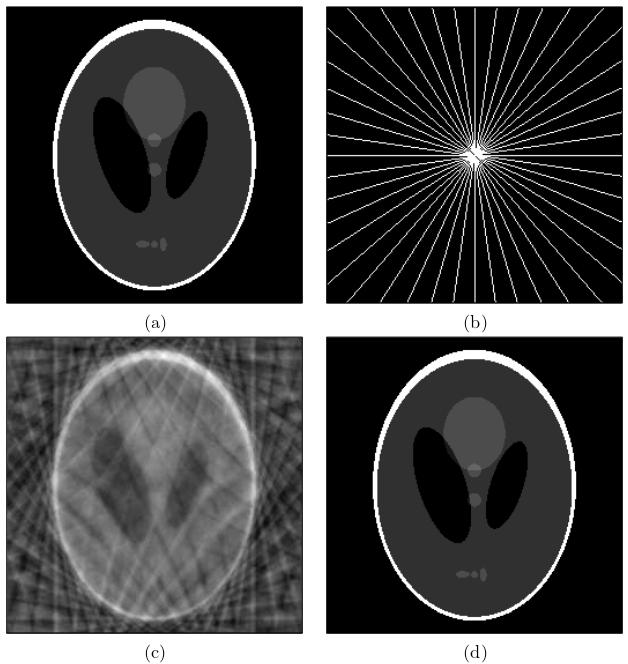
\includegraphics[width=0.6\textwidth]{img/candesmri}
    \end{center}
    \legend{Fonte: \citet{CandesMRI}}
    \label{fig:l1ball}
\end{figure}

\subsection{Resultados com dicionários coerentes}
A utilização de matrizes de amostragens incoerentes, ou dicionários incoerentes, limita a aplicação de 
Compressed Sensing em algumas áreas, ou para alguns problemas cuja base de solução dos mesmos era baseada
em dicionários coerentes, que podem ser, por exemplo, um dicionário supercompleto, com mais colunas que linhas. 
"Coerência é, de certa forma, uma propriedade natural para Compressed Sensing, 
porque se duas colunas são muito correlatas, será impossível em geral distinguir se a energia do sinal
vem de uma ou da outra" 
\footnote{"Coherence is in some sense a natural property in the compressed sensing framework, for if two
columns are closely correlated, it will be impossible in general to distinguish whether the energy in 
the signal comes from one or the other"}
(\citeauthor{CANDESDICTS}, \citeyear{CANDESDICTS}, tradução própria).

Porém, em alguns casos, não precisa-se recuperar os coeficientes originais do sinal, o que com dicionários 
coerentes não é possível, mas sim o próprio sinal já transportado para uma nova base.
Matematicamente falando, imagine-se um sinal $\vec{f} = \mathbf{D}\vec{x}$, no qual suas medidas são
$\vec{y} = \mathbf{\Phi}\vec{f} = \mathbf{\Phi}\mathbf{D}\vec{x}$, se o dicionário $\mathbf{D}$ for
coerente, não é possível recuperar os coeficientes $\vec{x}$, mas é possível recuperar $\vec{f}$ \cite{CANDESDICTS}.

A partir desses estudos, \citet{CANDESDICTS} gerou uma nova definição para o problema de CS, 
baseado na solução utilizando a norma $\ell_1$, considerando $\vec{f} = \mathbf{D}\vec{x}$ o sinal
e $\vec{y} = \mathbf{\Phi}\vec{f} + \vec{e}$ as medidas, $\vec{e}$ o erro.
\begin{equation}
    \label{eq:problemDl1}
    \vec{f'} = \underset{\vec{g} \in \mathbb{C}^d}{\text{argmin}} \lVert \mathbf{D}^*\vec{g} \rVert_1 
    \hspace{1em} \text{sujeito a} \hspace{1em}
    \lVert \mathbf{\Phi} \vec{g} - \vec{y} \rVert_2 \le \epsilon
\end{equation}
tal que $\lVert \vec{e} \rVert_2 \le \epsilon $.

\citet{CANDESDICTS} também redefiniu a RIP, chamando de D-RIP como segue. 
Dado um operador de amostragem $\mathbf{\Phi}$, ele satisfaz a D-RIP para um determinado 
dicionário $\mathbf{D}$ de ordem $s$ se:
\begin{equation}
    (1 - \delta_s)\lVert \mathbf{D}\vec{x} \rVert\SPSB{2}{2} \le \lVert \mathbf{\Phi} \mathbf{D}\vec{x} \rVert \SPSB{2}{2} \le 
    (1 + \delta_s)\lVert \mathbf{D}\vec{x} \rVert\SPSB{2}{2} \hspace{1em} \text{para todo vetor s-esparso } \vec{x}.
\end{equation}
para algum $\delta_s$, por exemplo $\delta_s \le 0,08$.

Tomando a nova definição, \citet{CANDESDICTS} provou o seguinte teorema sobre a recuperação do sinal.
\begin{teorema}
    \cite{CANDESDICTS}
    Dado $\mathbf{D}$ um dicionário e supondo um operador de amostragem $\mathbf{\Phi}$ que satisfaz
    a D-RIP de ordem $s$.
    Então, a solução $\vec{f'}$ para a análise $\ell_1$ satisfaz:
    \begin{equation*}
        \lVert \vec{f'} - \vec{f} \rVert_2 \le C \left[ \epsilon + \frac{\lVert \mathbf{D}^* \vec{f} - \left( \mathbf{D}^* \vec{f} \right)_s \rVert_1}{\sqrt{s}} \right],
    \end{equation*}
    tal que $\left( \mathbf{D}^* \vec{f} \right)_s$ denota o vetor com os $s$ maiores coeficientes em 
    magnitude de $\mathbf{D}^* \vec{f}$ e $C$ é uma constante tal que $C \ge 0$.
\end{teorema}

Esse novo campo de estudo abriu caminhos para novas análises e usos de CS para outros
problemas, antes não possível, além tornar possível utilizar os modelos e técnicas de CS
para outros campos do conhecimento.

% \subsubsection{Métodos utilizando \textit{Total Variation}}
% Decidir se terá ou não

\section{Aprendizado de Dicionários}
A área de aprendizado de dicionários, do inglês \textit{Dictionary Learning}, busca, através
dos dados já conhecidos de uma classe de sinais, prover novos dicionários nos quais os sinais 
serão capazes de se conformar com maior esparsidade. 
Sob o ponto de vista de CS, um dicionário $\mat{D}$ normalmente é escolhido de forma aleatória,
desde que satisfaça a RIP.
Aprendizado de dicionários, por outro lado, busca gerar modelos considerando os sinais envolvidos,
ou seja, dicionários que dependem dos dados, ou \textit{data-dependent dictionaries} \cite{chen2015compressed}.

Nas seções seguintes será explicitado o problema geral de aprendizado de dicionários, bem como 
um algoritmo que é capaz de de gerar um dicionário a partir de dados observados, e, por fim, 
uma aplicação focada em processamento de imagens.

\subsection{Problema Geral de Aprendizado de Dicionários}
Nessa seção será apresentado um modelo geral do problema que aprendizado de dicionários busca resolver.
De forma intuitiva, pode-se imaginar aprendizado de dicionários como se fosse desejado gerar 
um sub-dicionário da língua portuguesa a partir de uma grande quantidade textos, livros, todos 
eles separados por palavras.

Mais formalmente, suponha-se $\vec{x_1}, \vec{x_2}, ..., \vec{x_n} \in \mathbb{R}^L$
um conjunto finito de sinais de trainamento, e inteiros positivos $m, s$.
Deseja-se encontrar a matriz $\mat{D}$ e os s-esparsos vetores 
$\vec{\gamma_1}, \vec{\gamma_2}, ..., \vec{\gamma_n} \in \mathbb{R}^m$ os quais
$\mat{D}\vec{\gamma_i} \approx x_i$ para todo $i$. Dessa forma, pode-se escrever o problema
de aprendizado de dicionários utilizando a norma $\ell_2$ como segue  \cite{chen2015compressed}:
\begin{equation}
    \label{eq:dlgeneral}
    \underset{\mat{D}, \vec{\gamma_1}...\vec{\gamma_n}}{min} 
    \sum_{i=1}^{n} {\lVert  \vec{x_i} - \mat{D} \vec{\gamma_i} \rVert \SPSB{2}{2}}
    \hspace{1em} \text{tal que} \hspace{1em}
    \lVert \vec{\gamma_i} \rVert_0 \le s, \text{ para todo } i.
\end{equation}

Nesse caso, $\mat{D} \in \mathbb{R}^{L\times m}$ é o dicionário aprendido, enquanto os 
vetores $\vec{\gamma_i} \in \mathbb{R}^m$, com no máximo $s$ coeficientes não nulos, é a representação
linear de $\vec{x_i}$ em $\mat{D}$. O valor de $m$ pode ser maior que o de $L$, talvez para 
explorar alguma redundância, mas $s\ll L$. Ainda, sobre o problema \eqref{eq:dlgeneral}, para que as escolhas
de $\vec{\gamma_i}$ e $\mat{D}$ sejam únicas, pode-se forçar que as colunas de $\mat{D}$ tenham norma $\ell_2$
unitária \cite{chen2015compressed}. O valor $m$ é conhecido como o número de átomos do 
dicionário.

É importante notar que a função de erro de \eqref{eq:dlgeneral} usa norma $\ell_2$, mas pode ser trocada
por outra função de erro, como, por exemplo, a norma $\ell_1$ \cite{chen2015compressed}.

Também é possível formular o problema com um dado erro de aproximação $\epsilon$.
Nesse caso, pode-se reformular o problema de aprendizado de dicionários como segue \cite{chen2015compressed}.
\begin{equation}
    \label{eq:dleps}
    \underset{\mat{D}, \vec{\gamma_1}...\vec{\gamma_n}}{min} 
    \sum_{i=1}^{n} {\lVert \vec{\gamma_i} \rVert_0}
    \hspace{1em} \text{tal que} \hspace{1em}
    \lVert \vec{x_i} - \mat{D}\vec{\gamma_i} \rVert_2 \le \epsilon, \text{ para todo } i.
\end{equation}

Unificando as duas formulações \eqref{eq:dlgeneral} e \eqref{eq:dleps}, chega-se ao seguinte
\cite{chen2015compressed}.
\begin{equation}
    \label{eq:dlunica}
    \underset{\mat{D}, \vec{\gamma_1}...\vec{\gamma_n}}{min} 
    \sum_{i=1}^{n} {\lVert \vec{x_i} - \mat{D}\vec{\gamma_i} \rVert\SPSB{2}{2} + \lambda \lVert \vec{\gamma_i} \rVert_0}
\end{equation}

Porém, utilizando-se a norma $\ell_0$, o problema é usualmente NP-difícil. Dessa forma, pode-se gerar
uma reformulação somente trocando a norma $\ell_0$ pela norma $\ell_1$ \cite{chen2015compressed}.
\begin{equation}
    \label{eq:dlunical1}
    \underset{\mat{D}, \vec{\gamma_1}...\vec{\gamma_n}}{min} 
    \sum_{i=1}^{n} {\lVert \vec{x_i} - \mat{D}\vec{\gamma_i} \rVert\SPSB{2}{2} + \lambda \lVert \vec{\gamma_i} \rVert_1}
\end{equation}

Aprendizado de dicionários tem ligação com diversas outras áreas do conhecimento. 
Em especial, e que será utilizado no decorrer do desenvolvimento do trabalho, está sua ligação
com CS, da forma que foi explicitada no início da seção, e com processamento de imagens,
o que será melhor abordados na seção \ref{sec:codesparsa}.

\subsection{\textit{Online Dictionary Learning}}
\label{sec:odl}
Um dos principais algoritmos de aprendizado de dicionários, com aplicação em processamento de imagens
é o algoritmo \textit{Online Dictionary Learning (ODL)}. Um de seus principais diferenciais
se dá pela possibilidade de utilizar um conjunto de treinamente bastante volumoso com bom 
desempenho \cite{MairalOnlineDictLearn}.

O ODL, como o próprio nome retrata, é um algoritmo \textit{online}, ou seja, a cada nova iteração $t$
é gerada uma nova versão do dicionário $\mat{D_{(t)}}$ a partir de uma nova amostra $\vec{x_{(t)}}$.

Entrando mais a fundo na definição geral do algoritmo, tomado um chute inicial $\mat{D_{(0)}}$, as próximas
iterações $t \ge 1$ serão baseadas em $\mat{D_{(t-1)}}$ e $\vec{x_{(t)}}$. O novo dicionário $\mat{D_{(t)}}$ será
gerado a partir de dois passos. Primeiramente, deve-se encontrar o vetor de coeficientes $\vec{\gamma_{(t)}}$
relativos a $\vec{x_{(t)}}$ e $\mat{D_{(t-1)}}$, resovendo o problema de codificação esparsa a seguir \cite{chen2015compressed}.
\begin{equation}
    \vec{\gamma_{(t)}} = \underset{\vec{\gamma}}{argmin}
    \frac{1}{2} \lVert \vec{x_{(t)}} - \mat{D_{(t-1)}}\vec{\gamma} \rVert\SPSB{2}{2} +
    \lambda \lVert \vec{\gamma} \rVert_1
\end{equation}
sendo que $\lambda$ é um parâmetro de configuração do algoritmo. Esse problema pode ser resolvido algum dos 
algortimos discutidos na seção \ref{sec:csalgo}. Também é possível alterar-se a norma $\ell_1$ pela $\ell_0$,
de forma que algum algoritmo guloso de CS possa ser utilizado. O mesmo se dará para o passo seguinte.

No segundo passo do algoritmo, definimos o novo dicionário $\mat{D_{(t)}}$ através dos vetores de coeficientes
anteriores, $\vec{\gamma_{(1)}}, ..., \vec{\gamma_{(t-1)}}$, além de considerar o novo $\vec{\gamma_{(t)}}$.
Para facilitar, consideremos a matriz $\mat{X}$ com colunas $\vec{x_1},...,\vec{x_t}$ e a matriz $\mat{\Gamma}$
com colunas $\vec{\gamma_1},...,\vec{\gamma_t}$.
Dessa forma, e considerando que os valores de $\vec{\gamma_i}$ são fixos, pode-se formular o problema \cite{chen2015compressed}.
\begin{equation}
    \mat{D_{(t)}} = \underset{\mat{D}}{argmin}
    \frac{1}{t} \sum_{i=1}^t \lVert \vec{x_i} - \mat{D}\vec{\gamma_i} \rVert\SPSB{2}{2}.
\end{equation}

Processando o problema anterior, chega-se em que ele pode ser resolvido utilizando-se o método do 
gradiente descendente. Para isso, primeiramente precisamos definir as matrizes a seguir \cite{chen2015compressed}.
\begin{equation}
    \mat{A_{(t)}} = \sum_{i=1}^t \vec{\gamma_i}\vec{\gamma_i^T} \in \mathbb{R}^{m \times m},
    \hspace{0.5em}
    \mat{B_{(t)}} = \sum_{i=1}^t \vec{x_i}\vec{\gamma_i^T} \in \mathbb{R}^{L \times m}.
\end{equation}

Tomando como valor inicial $\mat{D} = \mat{D_{(t-1)}}$, e utilizando o seguinte cálculo em cada coluna $\vec{d_k}$, 
de forma iterativa,
que sempre minimiza a função objetivo, chega-se no novo dicionário $\mat{D_{(t)}}$.
\begin{equation}
    \vec{d_k} \leftarrow \frac{1}{\mat{A_{(t)_{k,k}}}}
    \left( \vec{B_{(t)_{:,k}}} - \mat{D}\vec{A_{(t)_{:,k}}} \right) +
    \vec{d_k}
\end{equation}

Por fim, será descrito o algoritmo do ODL, conforme \citet{MairalOnlineDictLearn}.

\begin{algorithm}[H]
    \label{algo:odl}
    \caption{\textit{Online Dictionary Learning (ODL)}}
    \Entrada{Distribuição de $\vec{x} \in \mathbb{R}^L = p(\vec{x})$, parâmetro $\lambda$, 
    dicionário inicial $\mat{D_{(0)}}$, número de iterações $T$.}
    \Saida{Dicionário final $\mat{D_{(t)}}$.}
    $\mat{A_{(0)}} \leftarrow \mat{0}$\;
    $\mat{B_{(0)}} \leftarrow \mat{0}$\;
    \For{$t = 1..T$}{
        Escolher nova amostra $\vec{x_{(t)}}$ de $p(\vec{x})$\;
        Resolver:
        $\vec{\gamma_{(t)}} = \underset{\vec{\gamma}}{argmin} \lVert \vec{x_{(t)}} - \mat{D_{(t-1)}}\vec{\gamma} \rVert_2^2 +
        \lambda \lVert \vec{\gamma} \rVert_1$\;
        $\mat{A_{(t)}} \leftarrow \mat{A_{(t-1)}} + \vec{\gamma_{(t)}} \vec{\gamma_{(t)}^T}$\;
        $\mat{B_{(t)}} \leftarrow \mat{B_{(t-1)}} + \vec{x_{(t)}} \vec{\gamma_{(t)}^T}$\;
        Realizar a atualização do dicionário para todas as colunas $k$ até convergência:
        $\vec{d_k} \leftarrow \frac{1}{\mat{A_{(t)_{k,k}}}}
        \left( \vec{B_{(t)_{:,k}}} - \mat{D}\vec{A_{(t)_{:,k}}} \right) + \vec{d_k}$ \;
        \If{$\lVert \vec{d_k} \rVert_2 > 1$}{
            Normalizar $\vec{d_k}$\;
        }
    }
    \Return{$\mat{D_{(t)}}$}
\end{algorithm}


\subsection{Codificação Esparsa}
\label{sec:codesparsa}
A partir das bases de Compressed Sensing e de aprendizado de dicionários, pode-se 
buscar um outro objetivo, compressão de sinais.
No caso que será estudado, o foco será em codificação esparsa de imagens, buscando 
embasar os estudos para a proposta do trabalho em questão.

É necessário considerar que imagens não são usualmente esparsas no domínio tempo.
Porém, no domínio da Transformada do Cosseno, ou no domínio da DCT, \textit{Discrete Cosine Transform}, 
imagens são, em geral, compressíveis, vide \eqref{eq:compressiblesignal}, fato 
que permite, por exemplo, gerar representações da imagem com alta fidelidade, mesmo
utilizando baixa quantidade de informação.
% Preciso de referências aqui.

Por outro lado, pode-se imaginar que, para uma determinada classe de imagens,
por exemplo, imagens naturais, a utilização de um dicionário previamente treinado 
pode gerar bons resultados. Para remoção de ruído em imagens, \citet{EladDenoising} 
mostram que o uso de dicionários aprendidos têm resultados melhores que o uso de 
dicionários gerais, teóricos.

Considerando uma imagem $I$, separada em patches $P_i$ de tamanho $\sqrt{L}\times\sqrt{L}$, 
com ou sem sobreposição - normalmente para problemas de remoção de ruído, com sobreposição,
enquanto para representação esparsa, sem - e vetorizando cada patch $P_i$ em vetores
$\vec{x_i} \in \mathbb{R}^L$. Tomando um dicionário $\mat{D} \in \mathbb{R}^{L\times m}$, 
aprendido via patches de imagens correlatas a $I$, se desejar-se representar os patches 
$\vec{x_i}$ em relação a $\mat{D}$, temos a seguinte formulação.
\begin{equation}
    \label{eq:patchcoding}
    \vec{\gamma_i} = \underset{\vec{\gamma}}{argmin} \lVert \vec{x_i} - \mat{D}\vec{\gamma} \rVert_2^2
    \hspace{1em} \text{sujeito a} \hspace{1em}
    \lVert \vec{\gamma} \rVert_0 \le s
    \text{ para todo } i,
\end{equation}
tal que $s$ é o número máximo de valores não nulos da representação $\vec{\gamma_i} \in \mathbb{R}^m$.
Para resolver essa formulação, pode-se utilizar algum dos algoritmos apresentados na
seção \ref{sec:greedy}, por exemplo o OMP. 
Para que a representação seja esparsa, precisa-se garantir que $s \ll L$.
Por exemplo, tomando uma imagem $I$ e separando em patches de $8\times 8$, ou seja,
$L = 64$, poderia ser escolhido um valor de $s = 8$ ou $s=12$, independente do valor 
de $m$, garantido $s < m$, cujo valor escolhido, por exemplo, poderia ser $m = 256$.

Existem diversas outras aplicações de aprendizado de dicionários no campo de processamento de
imagens, principalmente \cite{MairalSparse}:
\begin{itemize}
    \item \textit{Denoising}: remoção de ruído de imagens;
    \item \textit{Inpainting}: preenchimento de regiões não \textit{pintadas} de imagens;
    \item \textit{Demosaicking}: reconstrução da imagem a partir de sensores digitais;
    \item \textit{Up-scaling}: aumento da resolução de imagens.
\end{itemize}

Estas aplicações fogem ao escopo do trabalho apresentado, portanto não serão
aprofundadas nesse referencial, porém são amplamente desenvolvidas por diversos
autores da área.

% \section{Codificação de Imagens}
% Decidir se terá ou não

\section{Codificação de Huffman}
Dentre os diversos tipos de codificação de dados que existem, algumas delas 
permitem a representação compacta dos dados sem perdas de compressão.
Esse é o caso da codificação de Huffman, um algoritmo de compressão por entropia,
ou seja, que se aproveita da repetibilidade dos dados e de sua distribuição, 
pois, em geral, a informação possui bastante redundância.

O método foi apresentado em 1952, e continua sendo amplamente utilizado. 
Em primeiro lugar, considere-se que deseja-se comprimir uma sequência de 
símbolos, ou mensagem, utilizando códigos de tamanho variável, um para cada símbolo.
Segundo \citet{HuffmanCoding}, duas restrições básicas são impostas para 
a codificação de mensagens:
\begin{enumerate}
    \item Dois símbolos diferentes não podem ter o mesmo código;
    \item Os códigos das mensagem precisam ser construídos de forma que não seja necessário 
    identificar onde começa ou termina um código.
\end{enumerate}

Um princípio básico utilizado é que o tamanho de um código nunca pode ser menor 
do que o de outro menos provável \cite{HuffmanCoding}.

Para facilitar as explicações, dados $N$ símbolos, eles serão representados 
pelos numerais $1, 2, ..., N$.
Algo que pode ser assumido, sem perda de generalidade, considerando $P(s)$ a probabilidade de um símbolo
$s$ qualquer aparecer na mensagem, é que \cite{HuffmanCoding}:
\begin{equation}
    \label{eq:hufprob}
    P(1) \ge P(2) \ge \cdots \ge P(N).
\end{equation}

Por consequência, se quisermos uma codificação ótima, o tamanho do código $L(s)$ 
deve ser \cite{HuffmanCoding}:
\begin{equation}
    \label{eq:huflen}
    L(1) \le L(2) \le \cdots \le L(N).
\end{equation}

Pode-se definir, a partir de \eqref{eq:hufprob} e \eqref{eq:huflen} o tamanho $L$ da mensagem 
codificada:
\begin{equation*}
    L = \sum_{i=1}^N {P(i)L(i)}.
\end{equation*}

É importante ressaltar que:
\begin{equation*}
    \sum_{i=1}^N {P(i)} = 1.
\end{equation*}

Por fim, \citet{HuffmanCoding} apresentou três restrições iniciais resumidas, além das iniciais.
Considere-se $D$ o número de valores que um dígito do código pode assumir.
\begin{enumerate}
    \item $L(1) \le L(2) \le \cdots \le L(N-1) = L(N)$.
    \item Pelo menos $2$ e não mais que $D$ símbolos com código de tamanho $L(N)$ tem códigos 
    com início idêntico, diferenciando-se por seus dígitos finais.
    \item Cada possível sequência de $L(N)-1$ dígitos deve ser usada ou como código ou ser 
    prefixo de outros códigos.
\end{enumerate}

Em seguida, serão explicados os passos do algoritmo apresentado em \citet{HuffmanCoding}.
Por fim, será mostrado um exemplo.
Para facilitar, vamos utilizar o problema de codificação binária, $D=2$, com valores 
possíveis do dígito $0$ e $1$.

A explanação partirá de que a tabela das probabilidades de cada símbolo já está pronta.
Para gerar essa tabela, podem ser simplesmente contadas quantas vezes cada símbolo aparece
em relação ao total dos símbolos da mensagem.

Tomando a tabela de probabilidades ordenada, os dois símbolos de menor probabilidade 
têm seus sufixos definidos por $0$ e $1$.
Em seguida, esses símbolos podem ser considerados como apenas um, com probabilidade igual 
a soma das duas probabilidades. 
A tabela então é atualizada removendo-se os dois símbolos e adicionando o símbolo unido. 
O processo volta a ser executado, iterativamente, até que haja somente um símbolo que seja 
a união de todos com a probabilidade $1$.
Cada vez que é definido o sufixo, considere-se que é inserido a frente do sufixo anterior 
de cada símbolo o valor $0$ ou $1$.

O exemplo a seguir mostra o funcionamento do algoritmo de forma mais clara.
Na figura abaixo, são mostrados os passos da codificação exemplificados por 
\citet{HuffmanCoding}.

\begin{figure}[H]
    \caption{Execução dos passos de codificação de Huffman}
    \begin{center}
        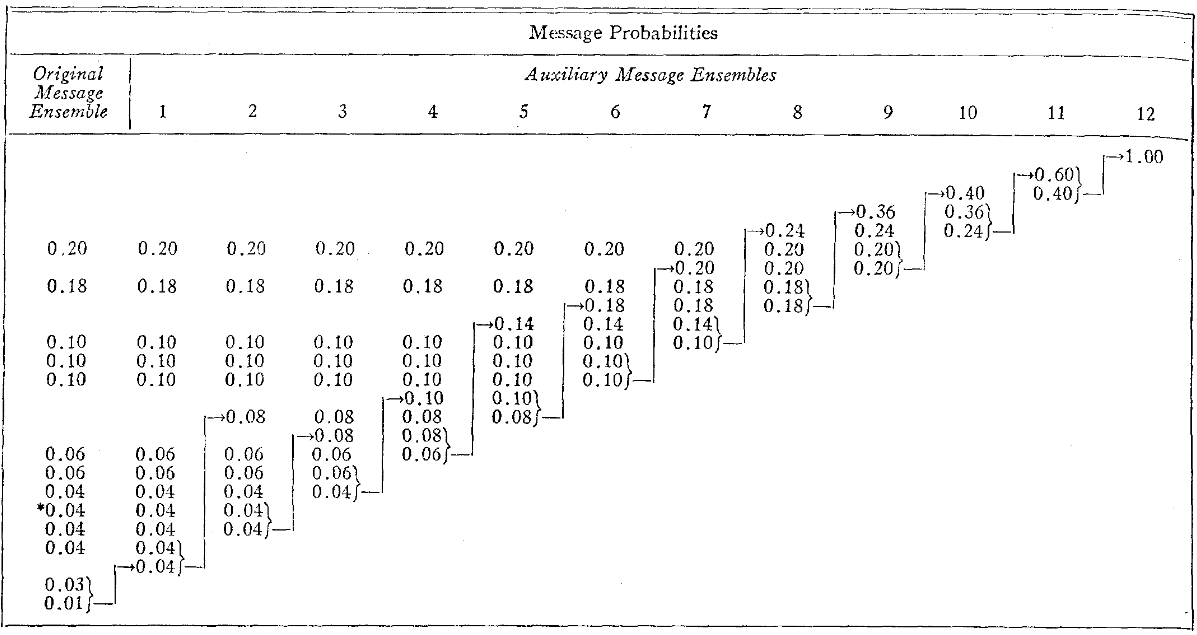
\includegraphics[width=0.9\textwidth]{img/huffmanprocess.png}
    \end{center}
    \legend{Fonte: \citet{HuffmanCoding}}
\end{figure}

Os códigos binários para cada símbolo gerados foram os seguintes:
\begin{figure}[H]
    \caption{Códigos binários gerados pela codificação de Huffman}
    \begin{center}
        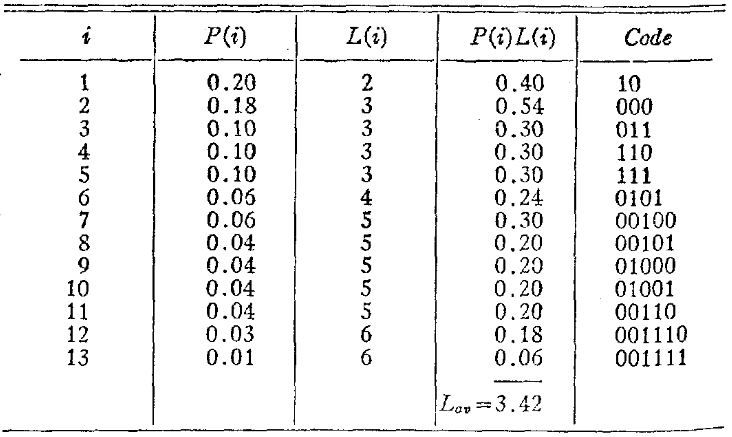
\includegraphics[width=0.6\textwidth]{img/huffmantable.png}
    \end{center}
    \legend{Fonte: \citet{HuffmanCoding}}
\end{figure}

O método apresentado é muito utilizado e possui variadas implementações na 
literatura.
Além disso, serve de base para diversos compressores de arquivos, também 
estando presente em padrões de codificação de imagens, tal qual o JPEG, 
ou de codificação de vídeo, por exemplo, o H.264.
% Escrever exemplo disso aí

\section{Codificação de Vídeo}
\label{sec:codvideo}
A comunicação através de vídeo, nas últimas décadas, tem sido uma das principais formas
de comunicação, sob as mais diversas formas.
\citet{SullivanH264} apresenta alguns cenários onde a vídeos digitais são aplicados:
\begin{itemize}
    \item Transmissão televisiva via satélite, ou cabo;
    \item Serviços de conversação via internet;
    \item Streaming de vídeos;
    \item Gravação e armazenamento de vídeos, por exemplo DVD.
\end{itemize}

Se imaginar-se armazenar, por exemplo, apenas uma imagem 720p, RGB, $1280\times720$, 
sem nenhuma compressão, utilizando $1$ byte por cor, a quantidade de bytes necessários 
para tal tarefa seria $1280\cdot720\cdot3 = 2764800$ bytes, ou, aproximadamente, $2,7Mb$
por imagem.
Expandindo a ideia, um vídeo de $10min$, ou $600s$, utilizando uma taxa de $30$ frames por segundo,
precisaria de quase $50Gb$ para ser armazenado!

Com esse pequeno exemplo, fica clara a necessidade de codificar os vídeos de forma a
reduzir substancialmente a quantidade de informação necessária para armazená-los.
A partir disso, serão descritas algumas características de \textit{codecs} 
(\emph{\textbf{co}der} e \emph{\textbf{dec}oder} de vídeo) precisam observar.

Um dos princípios básicos utilizados na codificação de vídeos é a de que o olho humano
é mais sensível ao brilho do que a cor diretamente \cite{SullivanH264}.
Ou seja, pode ser utilizada mais informação para representar o brilho, enquanto a cor
pode ser representada com menor precisão.
De fato é isso que acontece na maioria dos \emph{codecs}. 
Em geral, é utilizada o espaço de cor Y, Cb, Cr, no qual Y, chamado componente \emph{lumma},
ou o brilho, em geral é codificado com dimensão 4 vezes maior que Cb e Cr, componentes 
\emph{chroma} do cinza para o azul (Cb) e do cinza para o vermelho (Cr).

Em alguns \emph{codecs} de vídeo existe a possibilidade de utilizar os formatos
\emph{progressive} e \emph{interlaced} \cite{SullivanH264}.
No caso de \emph{progressive}, todo frame é salvo em sequência.
Já no formato \emph{interlaced}, podem ser utilizados campos entrelaçados.
Por exemplo, um primeiro campo pode ser as linhas pares do frame, enquanto o segundo
as linhas ímpares \cite{SullivanH264}.
No prosseguimento do texto será utilizado o termo imagem sem diferenciação entre os 
formatos apresentados.

Técnicas para compressão digital, não somente para vídeos, mas para aplicações em geral,
podem ser classificadas como segue \cite{SullivanH264}:
\begin{itemize}
    \item \textbf{Predição:} Processo no qual são criadas predições sobre a informação 
    que virá. Caso a predição for de boa qualidade, a diferença entre a predição e a 
    imagem em si, ou resíduo, será pequena, e, em geral, fácil de codificar, além de mais
    comprimida.
    \item \textbf{Transformações:} Este processo é o de buscar outras formas de representar
    os dados, em geral mais esparsas (ou comprimidas). Por exemplo, para imagens a DCT 
    fornece uma transformação mais compressível que a utilização da imagem bruta.
    \item \textbf{Quantização:} O processo de quantização se refere a representar os dados
    com menor quantidade de informação, ou seja, menos bits. Um exemplo é trocar uma representação 
    em ponto flutuante por uma representação em inteiros com 8bits.
    \item \textbf{Codificação de entropia:} Processo que utiliza a redundância de informação para 
    criar uma tabela de representação na qual a informação mais redundante é codificada
    com menos bits e a mais, com mais bits. A codificação de Huffman é um exemplo desse processo.
\end{itemize}

Uma forma simples de fazer compressão de vídeos se dá por tomar cada imagem do vídeos
separadamente e comprimi-la utilizando técnicas relativas a imagens, por exemplo JPEG \cite{SullivanH264}.
Ainda podem ser utilizadas técnicas de predição intra-frame, visando melhorar a codificação.
Essas técnicas atingem certo grau de compressão, porém vídeos possuem grande correlação temporal
entre seus frames, ou seja, o frame do instante $t$ está fortemente correlato ao frame $t-1$ e
ao frame $t+1$, em geral.
Utilizar a forma anterior não aproveita esse fato, o que leva a se imaginar buscar metodologias
que façam codificação inter-frame.

A imagem a seguir apresenta a ideia do funcionamento geral de um \textit{encoder} de vídeo,
mostrando, em conceito macro, o funcionamento do mesmo.
\begin{figure}[H]
    \caption{\textit{Encoder} de vídeo híbrido (em especial H.264).}
    \begin{center}
        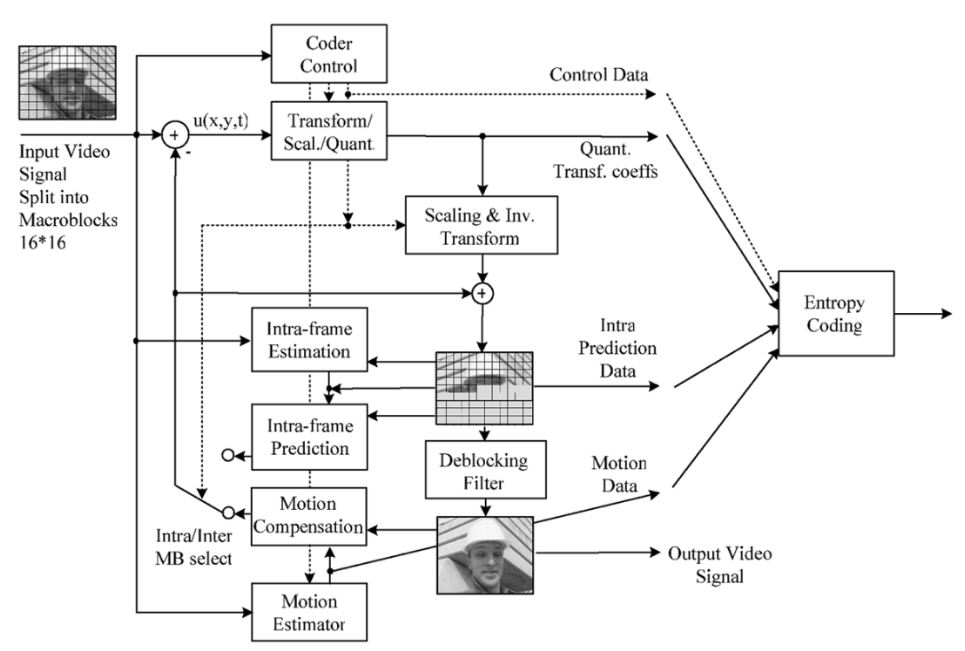
\includegraphics[width=0.7\textwidth]{img/HybridCodec.png}
    \end{center}
    \legend{Fonte: \citet{SullivanH264}.}
\end{figure}

Um conceito que aproveita a dependência temporal é o MCP (\textit{Motion-compensated prediction}).
O MCP considera que, muitas vezes, as mudanças durante os vídeos acontecem devido ao movimento.
Dessa forma, se for possível estimar um vetor de movimento, seria possível fazer uma predição
de compensação de movimento, uma estimativa de movimento \cite{SullivanH264}. 

Diversas formas de executar-se o MCP foram desenvolvidas pela literatura, unindo ganhos
na complexidade a ganhos em compressividade e qualidade, utilizando uma ou mais imagens 
do passado como base para criar predições de movimento.

A seguir será explicado, de forma superficial, o funcionamento do codec H.264, com o qual 
serão feitas comparações nesse trabalho.

\subsection{Codec H.264}
O codec H.264 foi lançado como padrão em 2003.
Ele incorporou funcionalidades de codecs anteriores, como H.262 e H.263, mas também
trouxe novas funcionalidades.

Antes de entrar mais especificamente nas funcionalidades, é necessário entender-se o 
funcionamento geral do codec.
Em primeiro lugar, podemos dividir o codec em network abstraction layer (NAL), a parte
relativa a configuração da rede pela qual o video será transmitido,
e a video coding layer (VCL), que diz respeito a forma como será representado o vídeo 
e seus frames.
Neste resumo o foco será nas funcionalidades relativas a codificação de vídeo, 
por tratarem de um assunto mais próximo a proposta do trabalho.

Sendo assim, a seguir serão listadas funcionalidades presentes no codec.
Basicamente, a VCL separa cada imagem porções com uma quantidade variável de macroblocos 
de dimensão $16\times16$.
Estes, por sua vez, podem ser divididos em sub-blocos de $16\times8$, $8\times16$,
$8\times8$, $8\times4$, $4\times8$ e $4\times4$.
A partir dos sub-blocos, dos macroblocos e das porções é que a codificação de vídeo 
é executada, levando em consideração o MCP.

Segundo \citet{WiegangH264}, as principais funcionalidades relativas a eficiência
da codificação são as seguintes:
\begin{itemize}
    \item \textbf{Motion Compensation (MC) com blocos de tamanho variável:}
    Dentro do macrobloco, cada um dos sub-blocos pode fazer MC.
    \item \textbf{MC com acurácia de um quarto de amostra:} A maioria dos codecs anteriores 
    provia MC com acurácia de um meio de amostra. O codec H.264 aumenta o poder 
    de acurácia para um quarto.
    \item \textbf{Vetores de movimento nas bordas da imagem:} Já presente como opcional
    no padrão H.263, permite que bordas também tenham vetores de movimento, utilizando
    técnicas de extrapolação das bordas.
    \item \textbf{Imagens de referência para MC múltiplas:} Permite que o \textit{encoder}
    escolha entre múltiplas imagens as referências para fazer MC.
    \item \textbf{Possibilidade de utilizar imagens preditas como referência:} Em alguns 
    codecs anteriores não era permitido utilizar imagens preditas como referência para o 
    processo de MC. O H.264 remove essa restrição.
    \item \textbf{Predição com pesos:} Permite que o MCP atribua pesos e offsets aos 
    sinais de referência utilizados.
    \item \textbf{Melhorias na predição intra-imagem:} Foram aprimoradas técnicas de
    extrapolação de arestas para a predição intra-imagem.
    \item \textbf{DCT aplicada a blocos menores:} No H.264 a DCT é aplicada a blocos de 
    dimensão $4\times4$, utilizando uma transformada inteira. Porém é possível aplicar 
    a DCT de mesma dimensão novamente a blocos maiores, de forma hierárquica.
    \item \textbf{Melhorias na codificação de entropia:} Foi melhorada a codificação de 
    entropia utilizando um método chamado \emph{arithmetic coding}.
\end{itemize}

Essa subseção buscou apresentar os conceitos básicos utlizados na codificação de vídeos, 
dando enfoque principal ao padrão H.264, fortemente utilizado no meio.
% Buscar terminar melhor essa parte....

\section{Introdução a CUDA\reg}
CUDA\reg~é uma plataforma de programação paralela, bem como um modelo de programação, 
desenvolvido pela NVIDIA para aplicações computacional em geral poderem ser executadas
em GPU's.
Sua primeira versão foi lançada em 2006.
Desde então, diversas empresas e trabalhos acadêmicos utilizaram a plataforma.
Além da forte utilização, também bibliotecas baseadas na plataforma surgiram, 
com o intuito de prover funções para aplicações já conhecidas como paralelizáveis.
Exemplos de tais plataformas são cuFFT, para aplicações com transformada de Fourier,
cuBLAS, para álgebra linear básica, NPP, para processamento de vídeo, imagens e 
sinais em geral.

A plataforma tem ótimos resultados para algoritmos, procedimentos, que possam utilizar
fortemente o paralelismo.
Atualmente, GPU's podem possuir mais de 4000 cores, por exemplo, a Nvidia Geforce RTX 2080 Ti,
além de serem capazes de rodarem 32 threads simultaneamente.
Todos os cores, ou pelo menos aqueles que forem designados para determinada aplicação,
devem estar rodando o mesmo código, porém com valores de variáveis que podem ser diferentes.

A arquitetura de CUDA\reg~se dá como na figura abaixo.
Ao ser executado um determinado \textit{kernel}, este é distribuído em um \textit{grid}
com $B$ blocos, cada blocs com $T$ threads.
Dentro de um bloco pode ser compartilhada memória de rápido acesso, enquanto para 
acesso fora do bloco precisa-se de memória global.
\begin{figure}[H]
    \caption{Arquitetura de CUDA\reg}
    \begin{center}
        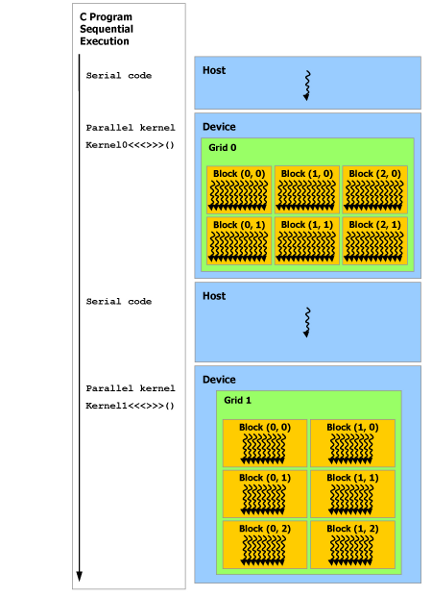
\includegraphics[width=0.5\textwidth]{img/CUDAarch.png}
    \end{center}
    \legend{Fonte: CUDA.....}
\end{figure}

Os resultados que CUDA\reg~apresenta são muito consistentes para algoritmos claramente
paralelizáveis, como é possível verificar no gráfico abaixo, que apresenta o 
\emph{speedup} alcançado por funções da cuBLAS em comparação com as mesmas funções 
executadas na CPU.
\begin{figure}[H]
    \caption{Speedup de cuBLAS (GPU) em relação a MKL BLAS (CPU)}
    \begin{center}
        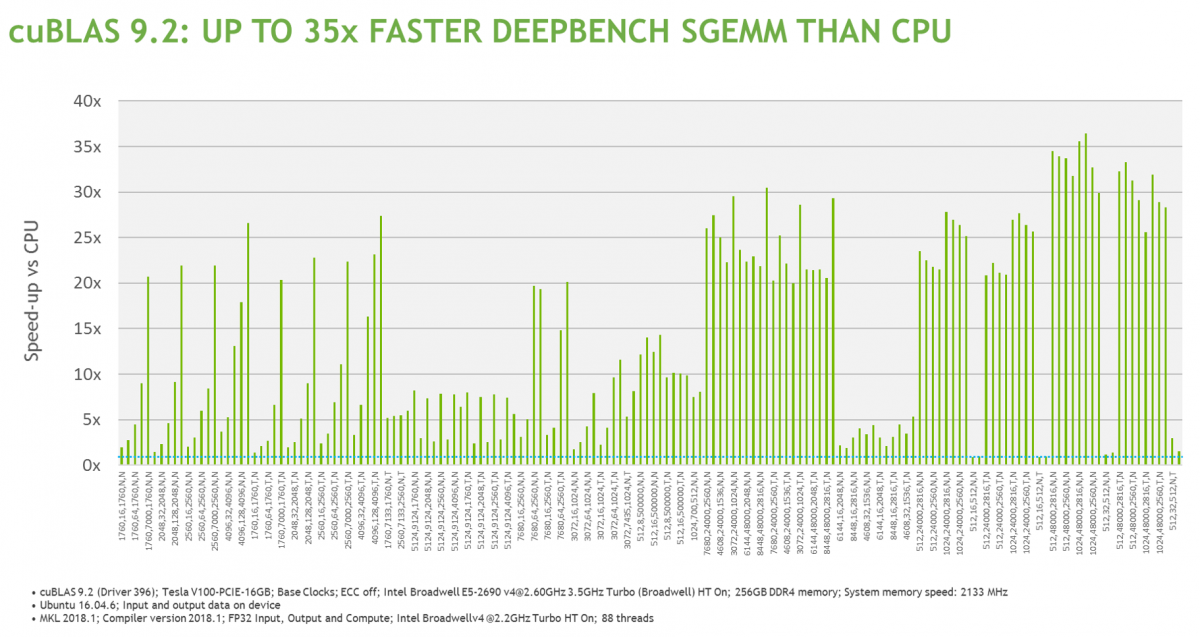
\includegraphics[width=0.9\textwidth]{img/cublas9_2.png}
    \end{center}
    \legend{Fonte: CUDA.....}
\end{figure}


Em geral o uso da interface com CUDA, através de alguma das linguagens de programação 
que permitem o uso, tais quais Python, C++, Fortran, se dá nas seguintes etapas:
\begin{enumerate}
    \item Alocação inicial de memória da GPU;
    \item Envio dos dados para a GPU;
    \item Processamento das informações;
    \item Aquisição dos dados;
    \item Liberação de memória da GPU.
\end{enumerate}

Os passos de alocação e liberação de memória demandam bastante tempo de CPU.
Em geral, para ganhos de performance, tenta-se alocar memória somente no início da
execução da aplicação, enviando, processando e recuperando as computações executadas 
sem gerar novas alocações.

Para exemplificar o quão simples é executar programas claramente paralelos em 
CUDA\reg, a seguir está descrito um \textit{kernel} que soma duas matrizes,
$\mat{A}$ e $\mat{B}$, colocando o resultado em $\mat{C}$.
\begin{center}
    \begin{lstlisting}
        __global__ void MatAdd(float A[N][N], float B[N][N],
                               float C[N][N])
        {
            int i = threadIdx.x;
            int j = threadIdx.y;
            C[i][j] = A[i][j] + B[i][j];
        }
        \end{lstlisting}
\end{center}

É possível perceber que, além da simplicidade do código, a sintaxe é muito próxima ao C. 
Esse fato pode ser considerado uma ajuda para a popularização da plataforma.
Também é possível verificar como se dá o paralelismo. 
Através dos parâmetros $x$ e $y$ de $threadIdx$, seleciona-se qual parte da matriz que 
será somada. 
Nesse caso, por simplicidade, é considerado que o \textit{kernel} será criado com apenas
$1$ bloco, de forma que somente é necessário utilizar o número da thread para definir 
os índices operados.

A plataforma CUDA\reg~foi utlizada no trabalho proposto para a paralelização do algoritmo
OMP (\ref{algo:omp}), conforme será discutido nos próximos capítulos.


\chapter{Trabalhos Relacionados}
Neste capítulo serão abordados alguns trabalhos que se relacionam com a proposta apresentada.
O foco principal da proposta está na codificação esparsa de frames de vídeos utilizando dicionários
previamente treinados, buscando executar o processo em tempo real.

Todos os trabalhos encontrados, bem como os padrões de vídeo existentes,
utilizam a técnida de separar os frames em blocos, ou \textit{patches},
para que a aplicação das técnicas de transformação e compressão sejam 
mais eficientes.

\citet{BRYTFACEKSVD}, em seu trabalho, fizeram a compressão de imagens de faces, 
utilizando o algoritmo K-SVD para aprendizado de um dicionário. 
Cada imagem facial foi amostrada para as mesmas dimensões, com as faces centralizadas
em um mesmo ponto, de forma que, aproximadamente, cada componente da face localiza-se
em uma mesma posição.
Por fim, cada imagem foi dividia e patches de tamanho $15\times 15$ sem sobreposição.
Para cada posição de patch, foi treinado um dicionário
de 512 átomos. A partir dessas definições, \citet{BRYTFACEKSVD} chegaram a resultados 
com alta taxa de compressão, e ótimas qualidades de recuperação da imagem.
Os resultados alcançados pelos autores indicam a possibilidade de se utilizar essa
metodologia de forma menos restritiva, com, possivelmente, resultados menos impressionantes
tanto em qualidade quanto em compressão.

Alguns trabalhos utilizam as teorias de CS para enviarem amostragens dos blocos
dos vídeos por parte do \textit{encoder}, utilizando-se dos teoremas provados pela teoria.
\citet{NebotDVC} apresentou um trabalho exatamente nesse sentido.
Seguindo o mesmo caminho, e buscando aprimorar a técnica apresentada por \citeauthor{NebotDVC}, 
\citet{DoDISCOS} propõe uma mescla entre os métodos tradicionais de codificação de vídeos
e a utilização de CS, conseguindo bons resultados e abrindo horizontes nesse sentido.
Em ambos trabalhos, a etapa de CS deve ser executada por parte do \textit{decoder}, 
o que é bastante custoso do ponto de vista de vídeos de maior resolução.

\citet{ZhangVideoCS} propõe um método que também mescla os métodos existentes
com a ideia de enviar amostragens. 
No trabalho proposto, apresenta uma forma de definir como cada bloco será codificado,
se utilizando amostragem ou DCT.
Os blocos que utlizam amostragem executam o processo de minimização da norma TV, 
enquanto os demais blocos aplicam a DCT inversa, por parte do \textit{decoder}.
A técnica foi incorporada a codificação H.264, chegando a ganhos significativos na
codificação \cite{ZhangVideoCS}.

Além destes trabalhos, o uso de CS para aprimorar vídeos de baixa qualidade foi 
apresentado por \citet{WirelessXiangCai}, com foco em distribuição de vídeos para
redes Wireless.
O uso de CS, nesse caso, se dá com o intuito de, além de melhorar os vídeos de baixa
qualidade e \textit{bitrate}, fornecer um canal capaz de lidar com ruído, 
tal qual a teoria de CS prevê.

Todos os trabalhos citados anteriormente utilizam como dicionário a DCT.
No sentido de utilizar técnicas de aprendizado de dicionários, 
\citet{chen2010dictionary} apresenta uma proposta baseada na de \citet{ZhangVideoCS},
porém, por parte do \textit{decoder}, ao invés de utilizar algum dicionário conhecida,
utilizar um aprendido.

% Ler o Lima e falar sobre com mais intensidade... OK
\citet{lima2012codificaccao} apresenta em seu trabalho um codec de vídeo bastante 
próximo ao proposto.
Em sua proposta, o autor utiliza o algoritmo K-SVD para treinamento de um dicionário
de 256 átomos, seguindo a proposta de \citeauthor{BRYTFACEKSVD}, conforme descrito
anteriomente.
Para a decomposição, também utiliza o algoritmo OMP, utilizando blocos $8\times8$,
sem sobreposição.
As principais diferenças entre o trabalho descrito e o proposto
estão no uso do ODL como algoritmo de treinamento de dicionários, 
além da forma como são processados os blocos.
No trabalho descrito, \citeauthor{lima2012codificaccao} utiliza a diferença entre o
bloco anterior e o atual ou somente o atual, dado um limite. 
No trabalho proposto, sempre será utilizado o bloco atual.
Porém, quando a diferença não for significativa, não recalculará a representação do bloco.
A escolha se dá pelo fato de que o dicionário base foi treinado para os blocos 
não residuais, e que, portanto, espera-se que a representação tenha melhores resultados 
para estes.

No próximo capítulo será detalhada a proposta do trabalho, explicitando detalhes
da implementação.
Em seguida, testes e resultados serão apresentados com base na proposta.

\chapter{Proposta}
Após considerar o desenvolvimento da área de CS e de aprendizado de dicionários e 
resumidos alguns trabalhos que focaram em alguma dessas áreas, será descrita a proposta 
do trabalho de forma detalhada.

O trabalho proposto visa desenvolver uma metodologia para codificação de vídeos em
tempo real, utilizando pré-aprendidos dicionários relacionados ao próprio vídeo.
Por ser um \textit{framework} com foco em tempo real, transmissão e recepção, 
naturalmente se põe em questão 
a necessidade de definir as funções que serão desenvolvidas por parte do \textit{encoder}
e por parte do \textit{decoder}.

% A proposta foca na codificação de frames a partir de dicionários previamente treinados,
% apresentando um novo olha sobre a transformação aplicada aos frames.
% As técnicas apresentadas de forma resumida na seção \ref{sec:codvideo} podem ser 
% aplicadas juntamente a metodologia apresentada.

A imagem a seguir apresenta um diagrama geral de blocos, dividindo entre \textit{encoder}
e \textit{decoder}, além de representar blocos funcionais de cada uma das partes de 
forma geral.
\begin{figure}[H]
    \caption{Diagrama geral da solução proposta}
    \begin{center}
        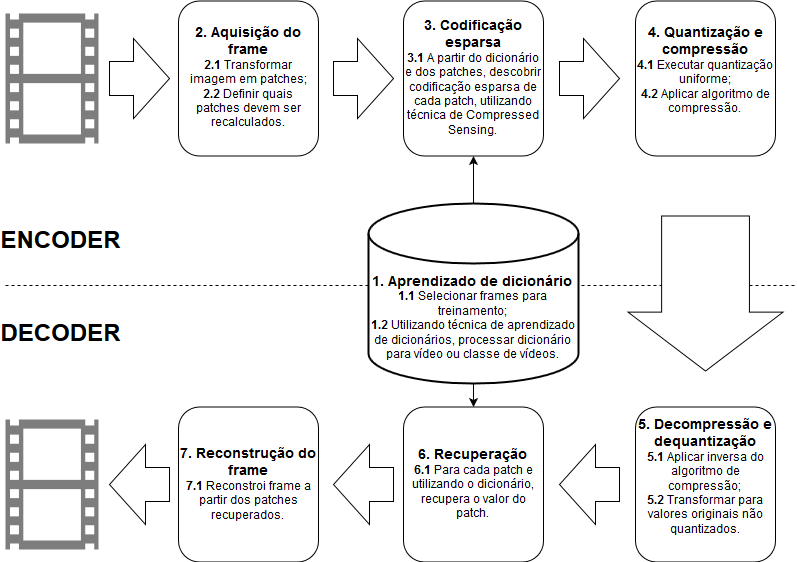
\includegraphics[width=0.9\textwidth]{img/DiagramaFinal.png}
    \end{center}
    \legend{Fonte: O Autor.}
\end{figure}

Entende-se que os frames processados estarão no formato de imagem colorida,
pixel a pixel, RGB (Red, Green, Blue). 
Ou seja, os frames terão dimensão 
$m \times n \times 3$,
sendo a resolução do vídeo $m \times n$. 
No caso do sistema criado, a ordem dos pixels é 
linha a linha, ou seja, primeiro a linha $0$ e todas suas colunas, depois a $1$, e assim por diante.
Em contraste com essa definição o frame em memória poderia ser coluna por coluna, o que alteraria
alguns cálculos internos, sendo possível adaptar o sistema desenvolvido de forma bastante simples.

Em seguida são definidas as nomenclaturas de alguns parâmetros importantes do
\textit{framework} proposto.

\section{Parâmetros do sistema}
Nessa seção serão mostrados os parâmetros do sistema que serão utlizados nas próximas
seções. 
As escolhas e resultados obtidos com a alteração dos parâmetros serão discutidas no 
capítulo \ref{sec:results}.

\begin{table}[h]
    \caption{Parâmetros do sistema}
    \centering
        \begin{tabular}{|c|p{10cm}|}
          \hline
          \multicolumn{1}{|c|}{\textit{Parâmetro}} & 
            \multicolumn{1}{c|}{\textit{Descrição}}\\
          \hline
          \hline
          $p$    & Tamanho do patch \\ 
          $s$    & Valor máximo de esparsidade de cada patch \\     
          $K$    & Número de átomos do dicionário \\
          $q$    & Esparsidade de envio da informação, $q \le s$ \\
          \hline
        \end{tabular}
    \legend{Fonte: O Autor}
    \label{tbl:params}
\end{table}

Nas seções seguintes serão descritas mais a fundo cada uma das etapas, seguindo a ordem
apresentada na imagem, além de explicitar a ligação entre cada um dos blocos funcionais
do projeto.

\section{Aprendizado de dicionário}
\label{sec:learn}
A parte de aprendizado do dicionário é essencial para que a qualidade da representação
esparsa utilizada seja boa.
Além disso, para o caso de treinamento a partir de frames de vídeos, caso em que se está
trabalhando, é também necessário fazer a escolha de um algoritmo que permita a utilização
de uma grande quantidade de dados de treinamento.

Considerando isso e o desempenho apresentado por \citet{MairalOnlineDictLearn}, foi escolhido
como algoritmo de treinamento do dicionário o \textit{Online Dictionary Learning},
descrito em \ref{sec:odl},
pois esse apresenta bom resultado para grande número de sinais de treinamento.

O treinamento foi executado da seguinte forma:
\begin{enumerate}
    \item Separados frames de vídeos de classe semelhante. Por exemplo, vídeos naturais, vídeos
    de esportes, \textit{cartoon}, etc...
    \item Os frames foram sorteados, de forma a garantir que um comportamento dos últimos frames
    não prepondere sobre todo o dicionário.
    \item Cada frame foi separado em patches com tamanho $p \times p$, sendo $p$ o tamanho de
    patch escolhido para o sistema. \textbf{CITAR RESULTADO COM ESCOLHA DE TAMANHO DE PATCH}.
    Para o treinamento, foram utilizados patches com sobreposição. Por fim, todos os patches
    foram vetorizados da mesma forma que em \ref{sec:frameaquisition}.
    \item Executado algoritmo do ODL, conforme Algoritmo \ref{algo:odl}.
\end{enumerate}

Vale ressaltar que para vídeos muito especializados, pode-se utilizar um treinamento
mais especializado. Por exemplo, uma transmissão esportiva, que seja de somente um tipo
de esporte, pode treinar um dicionário somente com frames desse determinado esporte.

A fase de aprendizado do dicionário, por envolver um tempo maior de processamento,
deve ser executada antes da transmissão de tempo real, por parte do \textit{encoder}.
Isso é possível, mesmo que não
se conheça a transmissão em si, mas se conheça que tipo de conteúdo será transmitido.

Um importante parâmetro que deve ser escolhido é o número de átomos $K$ do dicionário.
Escolhas de valores maiores tendem a proporcionar maior qualidade na representação do vídeo,
porém com perda de desempenho. No capítulo \ref{sec:results} serão mostrados resultados
de escolhas diferentes no número de átomos do dicionário.

Como parametrização do ODL, utiliza-se o valor $s$ como esparsidade desejada e
$K$ como número de átomos do dicionário.
O algoritmo ainda precisa saber o número de amostras que devem ser selecionadas aleatoriamente
de cada frame.
Para determinar isso, foram executados testes de qualidade com diversos valores
\textbf{CITAR RESULTADOS}.
Foi utilizada a implementação da biblioteca SPAMS \cite{SPAMS} do algoritmo ODL.

O resultado final desse etapa será um dicionário $\mat{D} \in \mathbb{R}^{3p^2 \times K}$,
que será utilizado nas etapas seguintes de codificação e decodificação.
Assim, portanto, em caso de uma transmissão de tempo real ou até mesmo se salvo em arquivo,
uma das primeiras informações que deve ser enviada é o dicionário que servirá de base
para a transmissão.


\section{\textit{Encoder}}
\subsection{Aquisição do frame}
\label{sec:frameaquisition}
Essa etapa tem como entrada o frame a ser codificado, sendo que o histórico de frames já
processados, para a posterior verificação de igualdade, está armazenado também neste
subsistema.

Já nesse ponto do processamento é necessário ter em vista o tamanho dos patches $p\times p$
que será utilizado. A escolha deve seguir o parâmetro definido na escolha do dicionário.
Valores típicos a serem escolhidos são $p=4$ ou $p=8$. No capítulo \ref{sec:results} serão 
discutidos resultados alcançados com ambas escolhas de tamanho de patch.

A escolha por processar patches se dá pela necessidade do processamento em tempo real, pois 
os algoritmos relacionados a CS dependem diretamente do tamanho
dos sinais envolvidos, do tamanho dos dicionários e da esparsidade.
Porém, o tamanho dos dicionários e a esparsidade precisam ser maiores conforme maior for 
o sinal, o que leva a um aumento de complexidade mais que linear com o aumento do tamanho dos
patches, além de uma utilização maior de memória para o dicionário.
Utilizar patches pequenos possibilita a paralelização dos cálculos.
No caso do trabalho que está sendo apresentado, em que o processamento dos patches, que será 
comentado na próxima seção, se dá utilizando a arquitetura da GPU, a utilização de maior 
paralelismo tende a aumentar a velocidade de processamento.
Como já comentado na seção \ref{sec:learn}, existe também um \textit{trade-off} entre 
diminuir o tamanho do patch e aumentar a compressão.

Tomada a imagem RGB $\mat{I}$ de dimensões $m \times n \times 3$, ela será separada em patches
$p \times p \times 3$, sem sobreposição. Por exemplo, um dos patches iniciará em $\mat{I_{0,0}}$
e terá parte em $p$ linhas e $p$ colunas, indo a $\mat{I_{p-1, p-1}}$. Em seguida, o próximo
patch iniciará em $\mat{I_{0, p}}$ e terminará em $\mat{I_{p-1, 2p-1}}$.
Nos finais de linha e de coluna, os valores de $m$ e $n$ podem não ser divisíveis por $p$,
o que gera um resíduo. Nesse caso foi adotada a solução que o padrão JPEG utiliza de repetir
o último pixel a esquerda para as colunas e o pixel acima para as linhas, até que chegue-se
a um patch $p \times p$.
Junto ao processo de tomada dos patches, estes são vetorizados, também no formato 
linha a linha, para cada pixel RGB.
Para um patch $\mat{P}$, os três primeiros valores do vetor corresponderão ao RGB de
$\mat{P_{0,0}}$. 
Os próximos três a $\mat{P_{0,1}}$, e assim por diante.
Como resultado final, pode-se dizer que a imagem $\mat{I}$ foi separada em 
\begin{equation*}
    T = \ceil*{\frac{m}{p}} \ceil*{\frac{n}{p}}
\end{equation*}
sinais de dimensão $L = 3p^2$. Pode-se escrever esses sinais como uma matriz 
$\mat{X}\in \mathbb{R}^{L\times T}$, 
na qual cada coluna $\vec{x_i}$ da matriz representa um dos patches vetorizados.
\begin{figure}[H]
    \caption{Funcionamento da vetorização do patch.}
    \begin{center}
        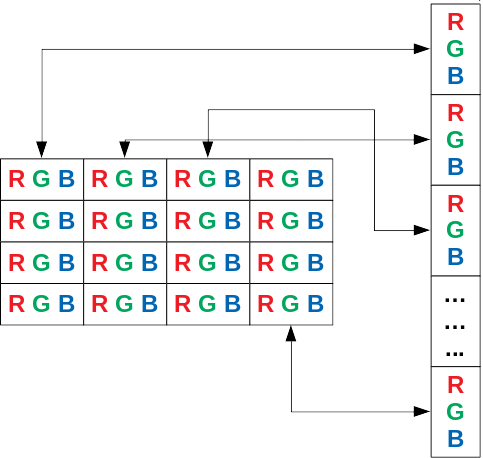
\includegraphics[width=0.6\textwidth]{img/vectorize}
    \end{center}
    \legend{Fonte: O Autor.}
\end{figure}

Além do processo de vetorização, este subsistema também verifica se o patch atual $i$ é 
igual ao mesmo $i$ anterior. Caso seja, marca um vetor $\vec{c}\in \mathbb{B}^T$, que indica os 
patches que precisam ou não ser recalculados.
A métrica considera que um patch deve ser recalculado caso qualquer um dos valores dos 
pixels inseridos nele mudem.
Esse simples cálculo sobre os patches garante que, para vídeos estáticos, o desempenho
da aplicação seja acelerado.
Grande parte dos vídeos possuem partes com essas características, e esse cálculo simples
não aumenta significativamente a complexidade do sistema como um todo.

\subsection{Codificação esparsa dos patches}
A partir dos patches $\mat{X}$ da etapa anterior, do dicionário $\mat{D}$, e do parâmetro 
de esparsidade desejada $s$, pode-se formular o problema de codificação esparsa, tal que 
$\vec{\gamma_i}$ seja a representação esparsa de $\vec{x_i}$, como segue:
\begin{equation}
    \vec{\gamma_i} = \underset{\vec{\gamma}}{argmin} \lVert \vec{x_i} - \mat{D}\vec{\gamma} \rVert_2^2
    \hspace{1em} \text{sujeito a} \hspace{1em}
    \lVert \vec{\gamma} \rVert_0 \le s,
    \text{ para todo } i.
\end{equation}

O problema acima, como citado anteriormente, pode ser resolvido via OMP.
A implementação básica escolhida para o sistema foi baseada na biblioteca SPAMS \cite{SPAMS}.
A partir dela, foi desenvolvida uma versão em CUDA, focada em paralelizar o algoritmo
OMP para cada $(\vec{x_i}, \vec{\gamma_i})$. Assim, foi possível calcular a representação
em tempo suficiente para transmissão em tempo real, conforme será verificado no capítulo 
de resultados \ref{sec:results}.

Um importante fato a ser considerado pelo algoritmo \ref{algo:omp} é que, a cada iteração,
ele descobre a melhor solução para essa esparsidade. Ou seja, se escolhida esparsidade $s=5$,
por exemplo, é possível armazenar-se os resultados com esparsidade $s=1,...,5$. 
A utlidade desse fato se dá no controle da taxa de transmissão, pois quanto mais esparsa a 
representação, menor a taxa. 
Portanto, com a aplicação do OMP, já se é possível gerar as melhores e piores representações.
Imaginando múltiplas transmissões a partir do mesmo \textit{encoder}, cada uma poderia ter 
uma taxa diferente sem a necessidade de mais cálculos nessa etapa.

Como resultado final desse subsistema teremos, para cada patch $i$, uma matriz de representação
$\mat{\Gamma_i} \in \mathbb{R}^{K \times s}$, sendo que cada coluna $(\mat{\Gamma_i})_j$ é 
j-esparsa.

\subsection{Quantização e compressão}
A partir da codificação esparsa apresentada na seção anterior, a ideia dessa seção é 
fazer com que a codificação seja a mais comprimida possível, sem perdas tão sensíveis
na representação do sinal.
Além disso, ao final dessa seção, é necessário que haja uma representação em formato de 
\textit{stream} de bytes, para ser enviada ou armazenada pelo \textit{encoder}.

Primeiramente, o sinal é quantizado uniformemente em 8bits. 
Para isso, é necessário identificar-se os coeficientes máximo $u$ e mínimo $l$ em $\mat{\Gamma}$.
Em seguida, cada coeficiente $c$ de $\mat{\Gamma}$ é quantizado de acordo com a seguinte equação:
\begin{equation*}
    c' = \floor*{0,5 + 255\frac{c - l}{u - l}}
\end{equation*}

Um dos parâmetros que entra em ação é o de esparsidade de envido da informação, $q$. 
Ele é o responsável pela escolha de qual será o nível de esparsidade escolhido,
dado que $1 \le q \le s$.
A partir desse parâmetro escolhem-se as colunas $q-1$ de cada $\mat{\Gamma_i}$ (já quantizado), 
formando $\mat{C} \in \mathbb{N}^{K \times T}$.
Para representação de $\mat{C}$ são utilizadas as matrizes $\mat{V} \in \mathbb{N}^{q \times T}$ e
$\mat{R} \in \mathbb{N}^{q \times T}$, sendo que $\mat{V}$ representa os coeficientes não nulos de
$\mat{C}$ e $\mat{R}$ representa os índices dos mesmos.

Para geração do \textit{bitstream}, são criados vetores a partir de $\mat{V}$ e $\mat{R}$.
Uma consideração importante é que nem sempre os $q$ índices de um patch estarão completos.
Nesse caso foi inserido um valor inválido no vetor de índices, enquanto o vetor de coeficientes
mantém os valores.

Como exemplo prático, selecione-se $q=3$ e $K=16$,
\begin{equation*}
    \mat{V} = 
    \begin{bmatrix}
        189 & 36 & 114 \\
        45  & -1 & 32  \\
        8   & -1 & -1
    \end{bmatrix},
    \mat{R} = 
    \begin{bmatrix}
        7 & 12 & 15 \\
        1  & -1 & 3  \\
        5   & -1 & -1
    \end{bmatrix}
\end{equation*}
tal que as entradas com valor $-1$ correspondem a entradas que não foram necessárias. 
Dessa forma, os vetores $\vec{v}$ e $\vec{r}$ serão os seguintes: 
\begin{center}
    $\vec{v} = \left[ 189, 45, 8, 36, 114, 32 \right]$, \\
    $\vec{r} = \left[ 7,1,5,12,-1,15,3,-1 \right]$.
\end{center}

Ainda em tempo, considerando que alguns dos patches não foram recalculados, estes 
também não precisam ser reenviados. 
Para marcar em que ponto isso acontece foi utilizado o valor $-2$ em $\vec{r}$, 
seguido do número de patches não enviados.

Esses vetores, mais a informação de máximo, mínimo e $q$ precisam ser empacotados 
e comprimidos para enviar ao decoder.

\textbf{ESCREVER SOBRE COMPRESSÃO!!!}

\section{\textit{Decoder}}

\subsection{Decompressão e dequantização}
\label{sec:decdeq}

\textbf{ESCREVER SOBRE DECOMPRESSÃO!!!}

A partir do sinal decomprimido deve-se recuperar as matrizes $\mat{V}$ e $\mat{R}$
tomandos os vetores $\vec{v}$ e $\vec{r}$ recebidos.

Em seguida é necessário recompor os coeficientes quantizados 
executando a operação inversa a de quantização.
Considerando $c'$ cada coeficiente recebido, $u$ o maior valor e $l$ o menor, 
valores todos recebidos,
\begin{equation*}
    c = \frac{c' (u - l)}{255} + l
\end{equation*}

Por fim, é inicializada com zeros uma matriz $\mat{\Gamma} \in \mathbb{R}^{K \times T}$,
basta associar $\mat{\Gamma_{\mat{R_{:,i}}, i}} = \mat{V_{:,i}}$ para todo $0 \le i < T$.

Vale lembrar que alguns dos patches podem não ter sido recebidos. 
Essa informação deve ser passada adiante para que somente os patches modificados
sejam reprocessados.

Terminada essa etapa procede-se com a recuperação dos patches.

\subsection{Recuperação dos patches}
A recuperação dos patches por parte do \textit{decoder} é um processo muito simples,
pois incorre somente em uma multiplicação entre o dicionário $\mat{D}$ e a 
representação esparsa recebida $\mat{\Gamma}$.

De tal modo, pode-se definir que a matriz de patches $\mat{X} = \mat{D} \mat{\Gamma}$.
Uma simplificação que pode aumentar a velocidade da decodificação é não criar a matriz $\mat{\Gamma}$,
ou seja, utilizar as informações de $\mat{V}$ e $\mat{R}$ para formar $\mat{X}$. 
Esse procedimento tende a ser mais eficiente, pois quando formada a matriz $\mat{\Gamma}$, 
a maior parte dos coeficientes dessa matriz é nulo, por se tratar de uma representação esparsa.
Porém, aplicando uma multiplicação da forma natural, esse fato é desconsiderado e acabam
acontecendo mais operações de multiplicação do que o necessário.

\subsection{Reconstrução do frame}
A reconstrução do frame se dá exatamente da forma contrária a separação por patches.

Vale notar que alguns dos patches não precisarão ser atualizados.
Essa informação foi recebida pelo \textit{decoder} na etapa \ref{sec:decdeq} e repassada
até essa etapa.

Assim, cada um dos patches de $\mat{X}$, que estavam vetorizados, são novamente transformados
em matrizes de dimensão $p \times p \times 3$, e colocados em sua devida posição, formando
a imagem recebida $\mat{I}$ de dimensões $m \times n$.

\chapter{Resultados}
\label{sec:results}

\chapter{Conclusão}


% referências
% aqui será usado o environment padrao `thebibliography'; porém, sugere-se
% seriamente o uso de BibTeX e do estilo abnt.bst (veja na página do
% UTUG)
% 
% observe também o estilo meio estranho de alguns labels; isso é
% devido ao uso do pacote `natbib', que permite fazer citações de
% autores, ano, e diversas combinações desses

\bibliographystyle{abntex2-alf}
\bibliography{biblio}

\end{document}
